%        File: main.tex
%     Created: Tue Jan 17 11:00 AM 2017 E
% Last Change: Tue Jan 17 11:00 AM 2017 E
%

\documentclass{beamer}
\usetheme{Frankfurt}
\usepackage{common}

  \title{Aerothermodynamic Design Sensitivities for a Reacting Gas Flow Solver
  on an Unstructured Mesh Using a Discrete Adjoint Formulation}

  \author{ Kyle B. Thompson }
  \institute[North Carolina State University and NASA Langley Research Center]{
    Mechanical and Aerospace Engineering Department \\
    North Carolina State University
    \and
    Aerothermodynamics Branch \\
    NASA Langley Research Center}

% Date of the Oral Preliminary Exam
\date{Month Day, 2017}

% This turns off the navigation bar at the bottom of each frame
\beamertemplatenavigationsymbolsempty

\begin{document}
\setbeamertemplate{caption}{\raggedright\centering\insertcaption\par}
\begin{frame}
  \titlepage
\end{frame}
\begin{frame}
  \frametitle{Outline}
  \tableofcontents
\end{frame}
\section{Introduction}
\stepcounter{subsection}
\begin{frame}
  \frametitle{Introduction - Design}
  \begin{itemize}
    \item Gradient-based design optimization is based on the minimization of a target
      ``cost'' function by changing a set of design variables
    \item A CFD code can be coupled with a numerical optimization package to
      iteratively improve target aerothermodynamic quantities, by change inputs to
      the CFD code
  \end{itemize}
  \begin{figure}[h]
    \centering
    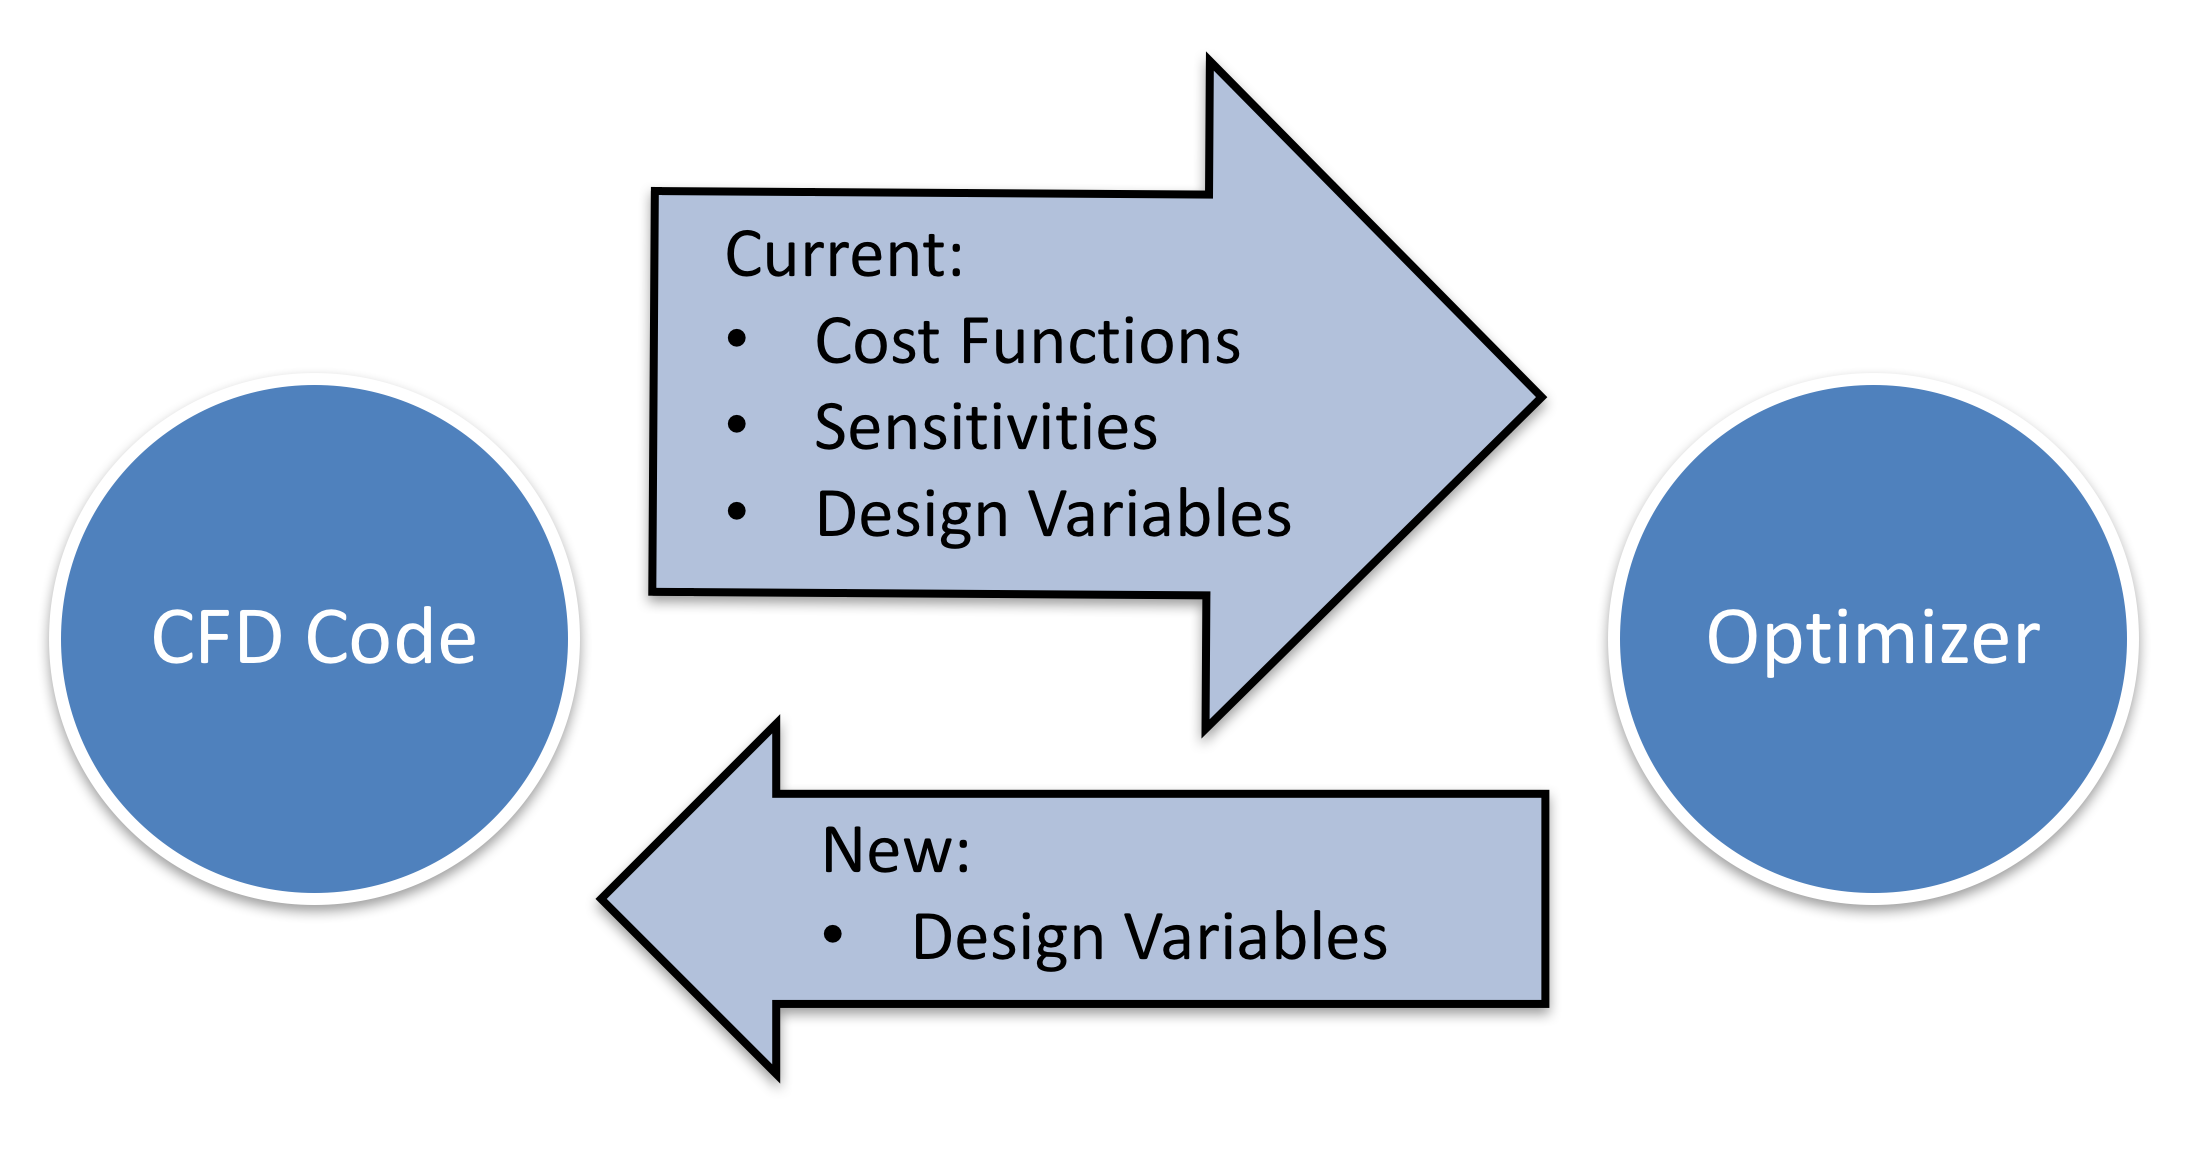
\includegraphics[width=0.6\textwidth]{figures/cfd-optimizer.png}
    \caption{CFD-Optimizer Relationship}
    \label{fig:cfd-opt}
  \end{figure}
\end{frame}
\begin{frame}
  \frametitle{Introduction - Design}
  \begin{itemize}
    \item The top-level design process is simple, but CFD sensitivity analysis 
      is expensive
    \item<2-> Need efficient way to compute cost function sensitivities for
      large number of design variables
  \end{itemize}
  \only<3>{\begin{tcolorbox}[colback=red!5!white,colframe=red!75!black, 
    title = Direct differentiation approach - Expensive]
    \begin{itemize}
      \item Navier-Stokes equations can be directly differentiated to yield
        sensitivity derivatives necessary for gradient-based optimization
      \item Finite difference requires a minimum of \textbf{one flow solution
        for each design variable sensitivity}
      \item Prohibitively expensive for large number of design variables
    \end{itemize}
  \end{tcolorbox}}
  \only<4>{\begin{tcolorbox}[colback=green!5!white,colframe=green!75!black,
    title = Adjoint approach - More efficient]
    \begin{itemize}
      \item Solve adjoint equations in addition to Navier Stokes flow equations to
        obtain sensitivity derivatives
      \item \textbf{One flow and adjoint solution needed for each cost function},
      regardless of number of design variables
      \item Considerably more efficient than direct differentiation approach for
        large number of design variables
    \end{itemize}
  \end{tcolorbox}}
\end{frame}
\begin{frame}
  \frametitle{Introduction - Design}
  \begin{itemize}
    \item Adjoint-based design optimization is widely adopted in compressible,
      perfect gas CFD solvers
    \item Reacting flow solvers have lagged in adopting adjoint-based approach,
      due to
    \begin{enumerate}
      \item Complexity of linearizing the additional equations for
        multi-species chemical kinetics
      \item Resorting to Automatic Differentiation tools incurs performance
        overhead that is implementation-specific
      \item Serious memory and computational cost concerns when simulating a
        large number of species
    \end{enumerate}
    \item Points 1 and 2 can be overcome through stubbornness (or hiring a
      graduate student\dots)
    \item Point 3 is a serious concern, if reacting flow solver are to be made
      attractive for design optimization
  \end{itemize}
\end{frame}
\begin{frame}
  \frametitle{Introduction - Improvement to State of the Art}
  \begin{itemize}
    \item Current state of the art
      \begin{itemize}
        \item Attempts made at both continuous\fcite{Copeland} and
          discrete\fcite{Lockwood} adjoint formulations
          for a compressible reacting flow solver
        \item These attempts suffer from quadratic scaling in memory and
          computational cost with number of species
        \item Recent scheme at Barcelona Supercomputing
          Center\fcite{Esfahani:2016aa} is promising, but only for
          incompressible reacting flows
      \end{itemize}
    \item Improvement to the state of the art
      \begin{itemize}
        \item New decoupled scheme for both hypersonic flow solver and adjoint
          solver that is robust for high-speed flows in chemical non-equilibrium
        \item New schemes significantly improve scaling in computational cost
          and memory with number of species
      \end{itemize}
  \end{itemize}
\end{frame}
\begin{frame}
  \frametitle{Introduction - Decoupled Approach}
  \begin{itemize}
    \item Reacting gas simulations require solving a large number of conservation
      equations
    \item Memory concerns
    \begin{itemize}
        \item Size of Jacobians scales quadratically with number species in gas mixture
        \item Solving system of equations in a tightly-coupled fashion can be
          limited by memory constraints
    \end{itemize}
    \item Cost concerns
    \begin{itemize}
      \item Cost of solving the linear system scales quadratically with number
      of species in gas mixture
    \end{itemize}
    \item Efficiently solving adjoint problem is a primary motivator
      \begin{itemize}
        \item Solving adjoint system particularly costly if linear solver is
          slow
        \item Can be necessary to store jacobian twice $\to$ large memory
          overhead
      \end{itemize}
  \end{itemize}
\end{frame}
\begin{frame}
  \frametitle{Introduction - Decoupled Approach}
  \begin{itemize}
    \item Loosely-coupled solvers have become popular in the combustion
      community\fcite{Sankaran}
      \begin{itemize}
        \item Decouple species conservation equations from meanflow equations,
          and solve two smaller systems
         \[
           \underset{(4+ns) \times (4+ns)}
           {\begin{pmatrix}
             \boxempty & \boxempty & \dots  & \boxempty \\
             \boxempty & \boxempty & \dots  & \vdots \\
             \vdots    & \vdots    & \ddots & \vdots \\
             \boxempty & \dots     & \dots  & \boxempty
           \end{pmatrix}}
           \to
           \underset{5 \times 5}
           {\begin{pmatrix}
             \boxempty & \dots  & \boxempty \\
             \vdots    & \ddots & \vdots \\
             \boxempty & \dots  & \boxempty
           \end{pmatrix}}
           \text{and}
           \underset{ns \times ns}
           {\begin{pmatrix}
             \boxempty  & \boxbslash & \dots  & \boxbslash \\
             \boxbslash & \boxempty  & \dots  & \vdots \\
             \vdots     & \vdots     & \ddots & \vdots \\
             \boxbslash & \dots      & \dots  & \boxempty
           \end{pmatrix}}
         \]
    \end{itemize}
  \item Candler, et al.\fcite{candler} originally derived this for
    Steger-Warming scheme, this work extends to Roe FDS scheme
  \end{itemize}
\end{frame}

\AtBeginSection[]
{
 \begin{frame}<beamer>
 \frametitle{Outline}
 \tableofcontents[currentsection]
 \end{frame}
}
\section{Flow Solver}

\subsection{Fully-Coupled Method}
\stepcounter{subsection}
\begin{frame}
  \frametitle{Fully-Coupled Point Implicit Method}
  \begin{itemize}
    \item All work presented is for inviscid flows in chemical non-equilibrium,
      using a one-temperature model, but is extendable to viscous flows.
    \item Beginning with the semi-discrete form
    \begin{equation*}
    	\label{inv_flux_fv}
    	\frac{\partial \mU}{\partial t}
    	 + \frac{1}{V}\sum\limits_{f}(\vF\cdot\ms)^f = \mw
    \end{equation*}
    \begin{equation*}
    	\begin{matrix}
    	\mU=\begin{pmatrix}
       		\rho_1\\
    		\vdots \\
    		\rho_{ns} \\
    		\rho u \\
    		\rho v \\
    		\rho w \\
    		\rho E \\
    	\end{pmatrix},      &
     	\mathbf{F \cdot S} = \begin{pmatrix}
    		\rho_1  \overline{U} \\
    		\vdots \\
    		\rho_{ns} \overline{U} \\
    		\rho u \overline{U} + p s_x\\
    		\rho u \overline{U} + p s_y\\
    		\rho u \overline{U} + p s_z\\
    		(\rho E + p) \overline{U} \\
    	\end{pmatrix}S,    &
     	\mw = \begin{pmatrix}
        \dot\rho_1\\
    		\vdots \\
    		\dot\rho_{ns} \\
        0 \\
        0 \\
        0 \\
        0
      \end{pmatrix}

  	\end{matrix}
  \end{equation*}

  \end{itemize}
\end{frame}
\begin{frame}
  \frametitle{Fully-Coupled Point Implicit Method}
  \begin{itemize}
  \item Using the Roe FDS scheme to compute the inviscid flux at the face,
    $\vF^f$, and linearizing the system results in
  \begin{multline*}
  	\frac{\mathbf{\delta U}^n}{\Delta t}
    +\frac{1}{V}\sum\limits_{f}(\frac{\partial \vF^f}
    {\partial \ul}\delta\mU^L
  	+\frac{\partial \vF^f}{\partial \ur}\delta\mU^R)^n \ms^f
  	- \frac{\partial \mw}{\partial \mU}\delta\mU^n \\
  	= -\frac{1}{V}\sum\limits_{f}(\vF^f\cdot\ms^f)^n + \mw^n
  \end {multline*}
  \item Which can be thought of more simply as
  \[
    \ma\vu = \vb
  \]
  \vspace{-0.7cm}
  \begin{align*}
    \ma &\to
    \begin{array}{c}
      (4+ns) \times (4+ns) \\
      \text{Jacobian Block}
    \end{array} \\
    \vb &\to
    \begin{array}{c}
      (4+ns) \times 1 \\
      \text{Residual}
    \end{array}
  \end{align*}
  \end{itemize}
\end{frame}
\begin{frame}
  \frametitle{Fully-Coupled Point Implicit Method}
  \begin{itemize}
    \item Constructing the Jacobian in a fully-coupled fashion results in large,
      dense block matricies
    \item Using a stationary iterative method (i.e., Gauss-Seidel, SSOR, etc.),
      work is dominated by matrix-vector products
      \[
        \text{Cost} \to O((4+ns)^2)
      \]
    \item Leads to onerous quadratic scaling with respect to number of species
  \end{itemize}
\end{frame}

\subsection{Decoupled Method}
\stepcounter{subsection}

\begin{frame}
  \frametitle{Decoupled Point Implicit Method}
  \begin{itemize}
    \item The main idea is to separate the meanflow and species composition
      equations, adding a new equation for the total mixture density
    \item Leads to two sets of conserved variables
      \begin{equation*}
      	\begin{matrix}
      		\mU'=\begin{pmatrix}
      			\rho \\
      			\rho u \\
      			\rho v \\
      			\rho w \\
      			\rho E
      		\end{pmatrix} &
      		\mathbf{\hat{U}}=\begin{pmatrix}
      			\rho_1 \\
      			\vdots \\
      			\rho_{ns}
      		\end{pmatrix} \\ \\
          \text{Meanflow} & \text{Species Composition}
      	\end{matrix} 
      \end{equation*}
  \end{itemize}
\end{frame}

\begin{frame}
  \frametitle{Decoupled Point Implicit Method}
  \begin{itemize}
    \item The fluxes are solved in two sequential steps
      \begin{itemize}
        \item  The mixture fluxes are first solved as
        \[
          \frac{\partial \mU'}{\partial t} +
          \frac{1}{V}\sum\limits_{f}(\vF'\cdot\ms)^f = 0
        \]
      \item Followed by the species fluxes
      \[
        \frac{\partial \mathbf{\hat{U}}}{\partial t} +
        \frac{1}{V}\sum\limits_{f}(\mathbf{\hat{F}}\cdot \ms)^f =
        \mathbf{\hat{W}}
      \]
    \end{itemize}
    \item Since the mixture density was determined in the first step, step two
      actually solves for the species mass fractions
      \begin{gather*}
        \delta \mathbf{\hat{U}}^n 
        = \rho^{n+1} \hat{\mv}^{n+1}-\rho^n\mathbf{\hat{V}}^n = \rho^{n+1} \delta
        \mathbf{\hat{V}}^n + \mathbf{\hat{V}}^n \delta \rho^n \\
        \mathbf{\hat{V}}=(c_1,\hdots,c_{ns})^T, c_s=\rho_s/\rho
      \end{gather*}
  \end{itemize}
\end{frame}
\begin{frame}
  \frametitle{Decoupled Point Implicit Method}
  \begin{itemize}
    \item The Roe FDS scheme species mass fluxes can be rewritten as
      \begin{align*}
  	\hat{\vF}_{\rho_s} &= c_s \vF'_\rho+(c_s^L-\tilde{c}_s)\rho^L\lambda^+
  	+ (c_s^R-\tilde{c}_s)\rho^R\lambda^- \\
	\frac{\partial \hat{\vF}_{\rho_s}}{\partial c_s^L} 
	&= w\vF_\rho+(1-w)\rho^L\lambda^+ - w\rho^R\lambda^- \\
	\frac{\partial \hat{\vF}_{\rho_s}}{\partial c_s^R} 
	&= (1-w)\vF_\rho+(w-1)\rho^L\lambda^+ + w\rho^R\lambda^- \label{d_last}
      \end{align*}
    \item Jacobian Approximations
      \begin{align*}
	\text{Step 1:}\quad &
	\frac{\partial \vF}{\partial \mU'}\bigg|_{\mathbf{\hat{V}}} =
	\underset{c_s = \text{Constant}}{5 \times 5\,\text{Roe FDS Jacobian}} \\
	\text{Step 2:}\quad & 
	\frac{\partial \vF}{\partial \hat{\mv}}\bigg|_{\mathbf{\hat{U'}}} = 
        \begin{pmatrix} 
          \frac{\partial F_{\rho_1}}{\partial c_1} & & 0
          \\ & \ddots &  \\ 0 & & \frac{\partial F_{\rho_{ns}}}{\partial c_{ns}}
        \end{pmatrix} 
      \end{align*}
  \end{itemize}
\end{frame}
\begin{frame}
  \frametitle{Decoupled Point Implicit Method}
  \vspace{-0.2cm}
  \begin{itemize}
    \item Chemical source term linearized via
    \vspace{-0.1cm}
    \begin{align*}
      \mathbf{\hat{W}}^{n+1} &= \mathbf{\hat{W}}^n+\frac{\partial
      \mathbf{\hat{W}}}{\partial \mathbf{U}}\bigg|_{\mathbf{U}'} \frac{\partial
      \mathbf{U}}{\partial \mathbf{\hat{V}}} \\
       \mc &= \frac{\partial \mathbf{\hat{W}}}{\partial
       \mathbf{U}}\bigg|_{\mathbf{U}'} \frac{\partial \mathbf{U}}{\partial
       \mathbf{\hat{V}}}
    \end{align*}
    \item Full system to be solved in step two
    \vspace{-0.2cm}
    \begin{gather*}
      \begin{split} \rho^{n+1}&\frac{\delta \hat{\mv}^n}{\Delta t}
        +\frac{1}{V}\sum\limits_{f}(\frac{\partial \hat{\vF}^f}{\partial
        \mv^L}\delta \mv^L +\frac{\partial
        \hat{\vF}^f}{\partial \hat{\mv}^R}\delta
        \hat{\mv}^R)^{n, n+1}\ms^f - \mc^{n, n+1}\delta\mv^n \\ &=
        -\frac{1}{V}\sum\limits_{f}(\hat{\vF}^{n,n+1}\cdot\ms)^f +
        \mw^{n, n+1} -\hat{\mv}^n\left(\frac{\delta \rho^n}{\Delta t} -
        R_\rho\right)
      \end{split} \\ 
    \end{gather*}
    \vspace{-1.4cm}
    \[
      R_\rho = -\frac{1}{V}\sum\limits_{f}{\sum\limits_{s}
      {(\hat{F}_{\rho_s}^{n,n+1}\cdot\mathbf{S})}}
    \]
  \item $R_\rho$ is included to preserve $\sum\limits_{s}{c_s}=1$, $\sum\limits_{s}{\delta c_s}=0$.
  \end{itemize}
\end{frame}

\section{Cost and Memory Savings}
\stepcounter{subsection}
\subsection{Cost and Memory Savings of the Decoupled Flow Solver}

\begin{frame}
  \frametitle{Cost and Memory Savings of the Decoupled Flow Solver}
\begin{itemize}
  \item Most significant savings comes from the source term linearization being purely node-based
    \begin{itemize}
      \item Convective contributions to block Jacobians are diagonal
      \item Source term jacobian is dense block Jacobian
      \item In the global system (w/chemistry), all off-diagonal block jacobians
        are diagonal
    \end{itemize}
  \end{itemize}
  \[
    \begin{pmatrix} 
      \Box & & & & \\ 
      & \ddots & & & \\ 
      & & \Box \\ 
      & & & \ddots & \\ 
      & & & & \Box
    \end{pmatrix} \begin{pmatrix} \delta \mathbf{\hat{V}}_1 \\ \vdots \\ \delta
      \mathbf{\hat{V}}_i \\ \vdots \\ \delta \mathbf{\hat{V}}_{nodes}
    \end{pmatrix} = \begin{pmatrix} \hat{b}_1 \\ \vdots \\ \hat{b}_i \\ \vdots \\
      \hat{b}_{nodes} \end{pmatrix} - \begin{pmatrix}
      (\sum_{j=1}^{N_{nb}}{[\diagdown] \delta\mathbf{\hat{V}}_{j}})_1 \\ \vdots \\
      (\sum_{j=1}^{N_{nb}}{[\diagdown] \delta\mathbf{\hat{V}}_{j}})_i \\ \vdots \\
      (\sum_{j=1}^{N_{nb}}{[\diagdown] \delta\mathbf{\hat{V}}_{j}})_{nodes}
    \end{pmatrix} 
  \]
  \begin{itemize}
    \item Matrix-vector products $\to$ inner products: $O(ns^2) \to O(ns)$
  \end{itemize}
\end{frame}
\begin{frame}
  \frametitle{Cost and Memory Savings of the Decoupled Flow Solver}
  \begin{itemize}
    \item Comparing size of Jacobian systems, using Compressed Row Storage
  \end{itemize}
  \begin{align*}
    \ma_d &= \text{Decoupled system Jacobians} \\
    \ma &= \text{Fully-coupled system Jacobians}
  \end{align*}
  \[
  \begin{split} Relative\ Memory\ Cost &=
    \frac{size(\ma_d)}{size(\ma)} \\ &= \lim_{ns\to\infty}
    \frac{(ns^2+5^2)(N_{nodes})+(ns+5^2)(N_{nbrs})}{(ns+4)^2(N_{nodes}+N_{nbrs})} \\
    &= \frac{N_{nodes}}{N_{nodes} + N_{nbrs}}
  \end{split}
  \]
\end{frame}

\subsection{Numerical Results: 2D Cylinder}

\begin{frame}
  \frametitle{Numerical Results: 2D Cylinder}
  \begin{figure}[h]
  	\centering
    \adjincludegraphics[width=0.8\textwidth,trim={0 7cm 0 7cm},clip]{figures/grid}
  \end{figure}
  \begin{itemize}
    \item Fully-coupled and decoupled methods both implemented in the Generic
      Gas Path of FUN3D
    \item Tested on 2D cylinder case
      \begin{itemize}
        \item $V_{\infty} = 5000\ m/s$, $\rho_{\infty}=0.001\ kg/m^3$, 
          and $T_\infty = 200\ K$
      \end{itemize}
    \item Inviscid flow, with 1-Temperature model
  \end{itemize}
\end{frame}

\begin{frame}
  \frametitle{Numerical Results: 2D Cylinder}
  \begin{itemize}
    \item Verification of implementation
    \begin{itemize}
      \item 5-species air model: N, $\text{N}_2$, O, $\text{O}_2$, and NO with five reactions
      \begin{columns}[t]
        \begin{column}{0.33\textwidth}
          \begin{figure}[h!]
            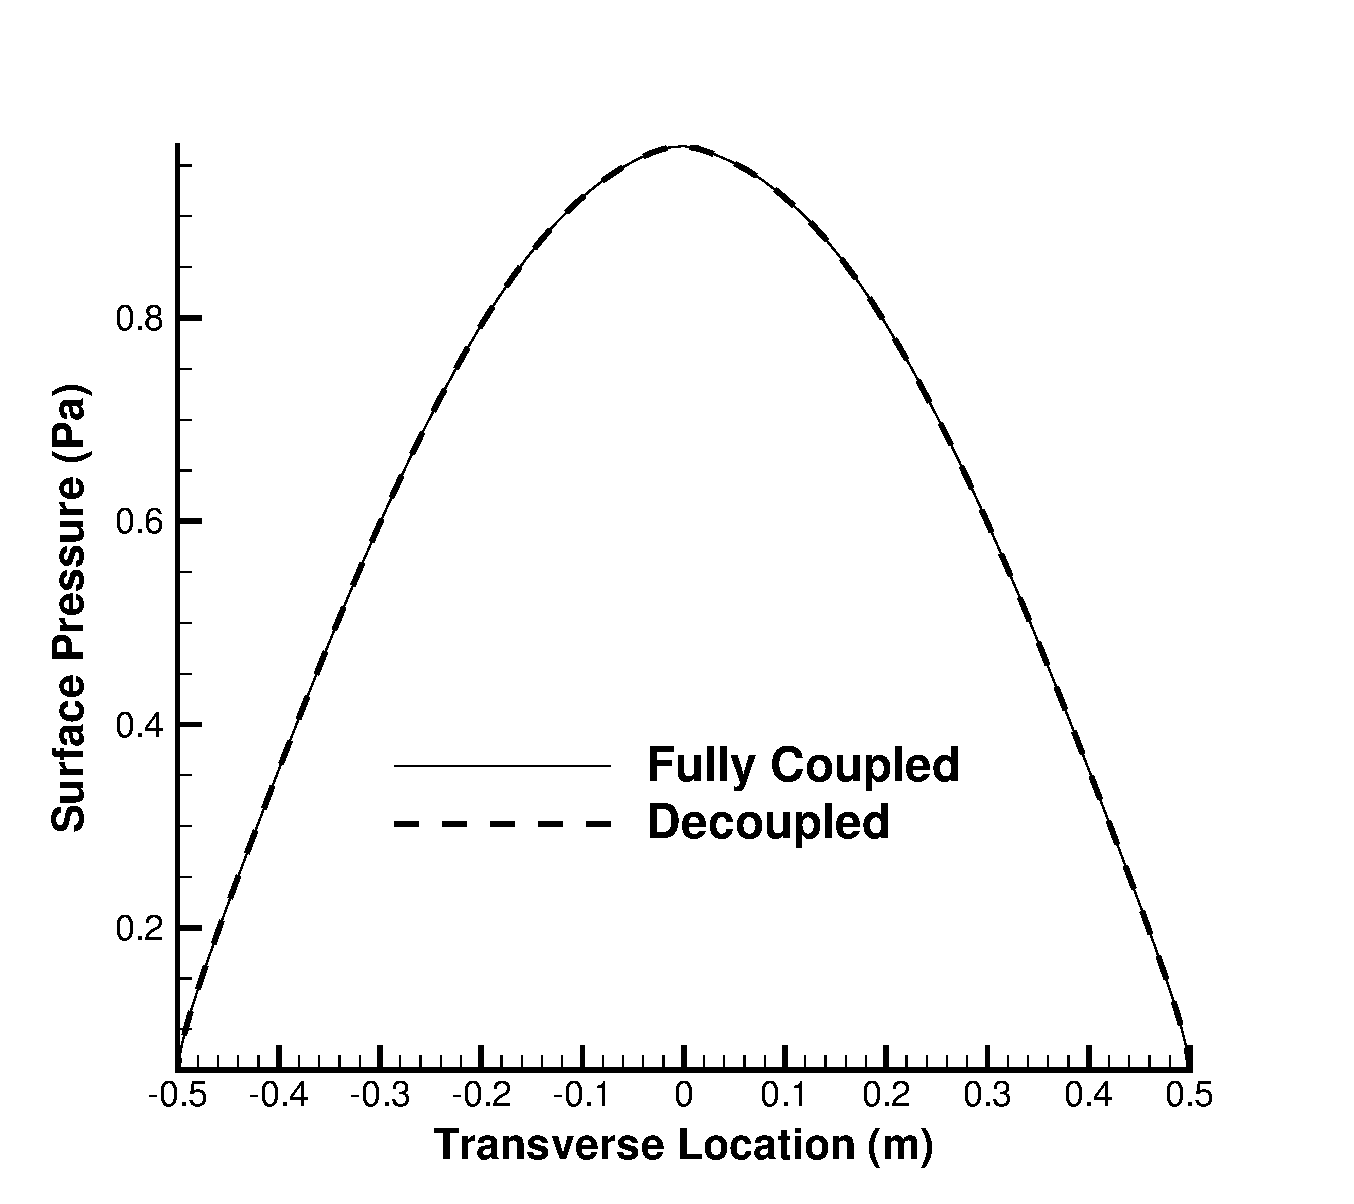
\includegraphics[width=\textwidth,trim={0 0 0 2cm}]{figures/surface_pressure}
          \end{figure}
        \end{column}
        \begin{column}{0.33\textwidth}
          \begin{figure}[h!]
            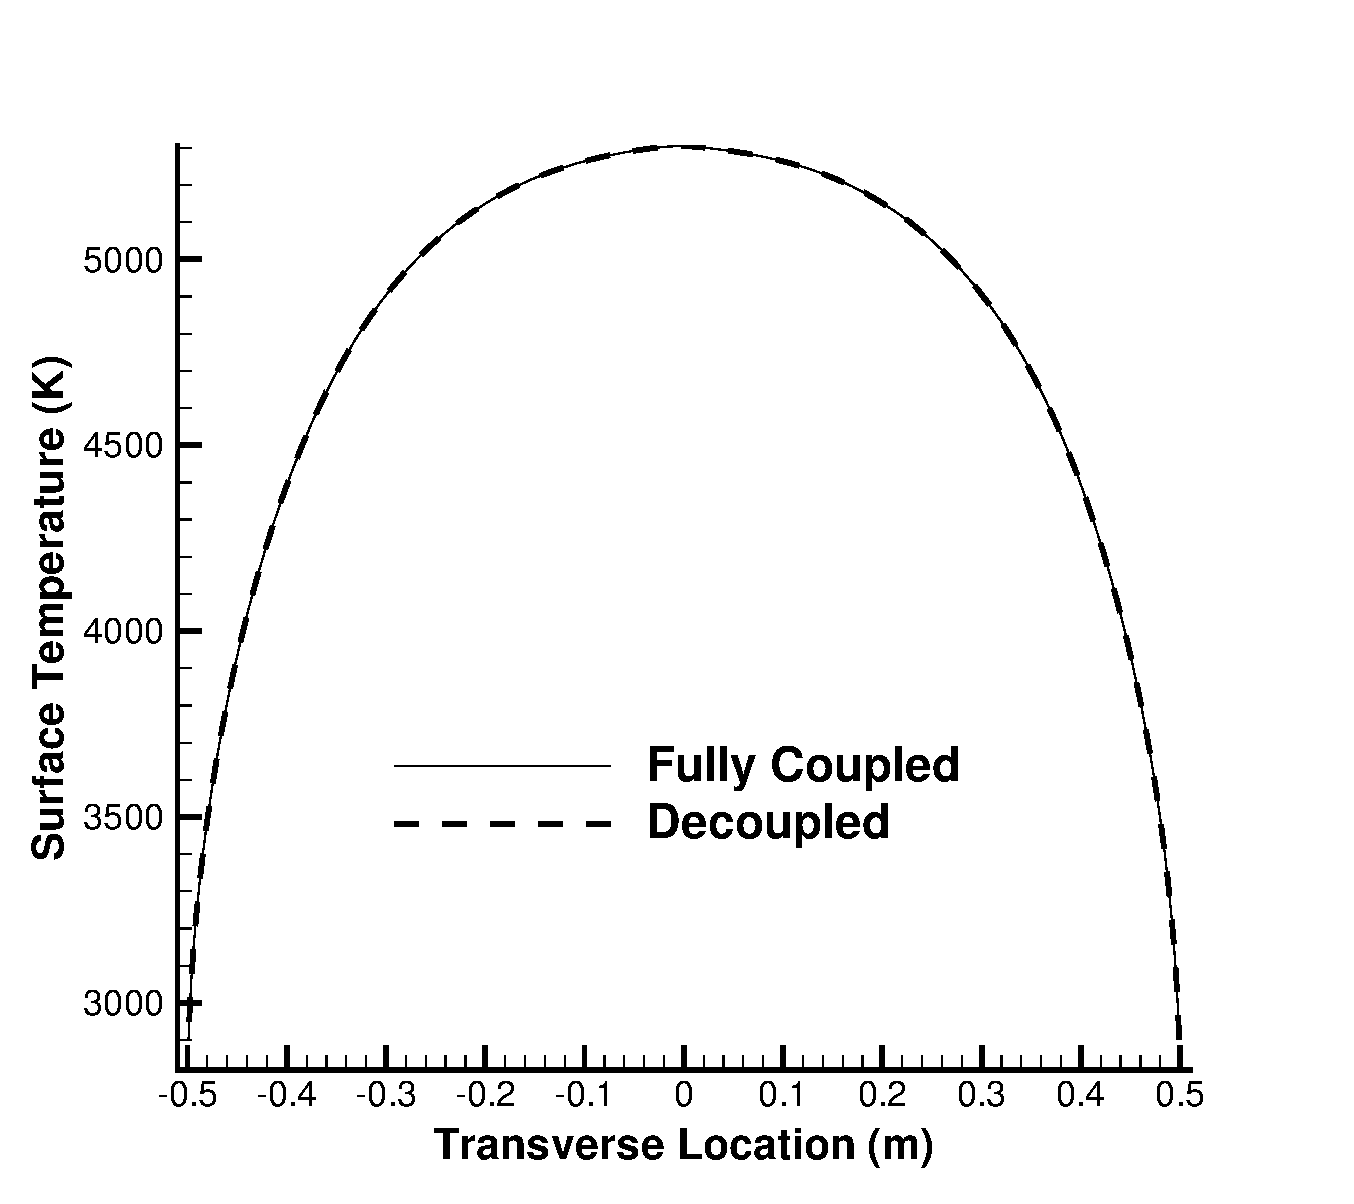
\includegraphics[width=\textwidth,trim={0 0 0 2cm}]{figures/surface_temperature}
          \end{figure}
        \end{column}
        \begin{column}{0.33\textwidth}
          \begin{figure}[h!]
            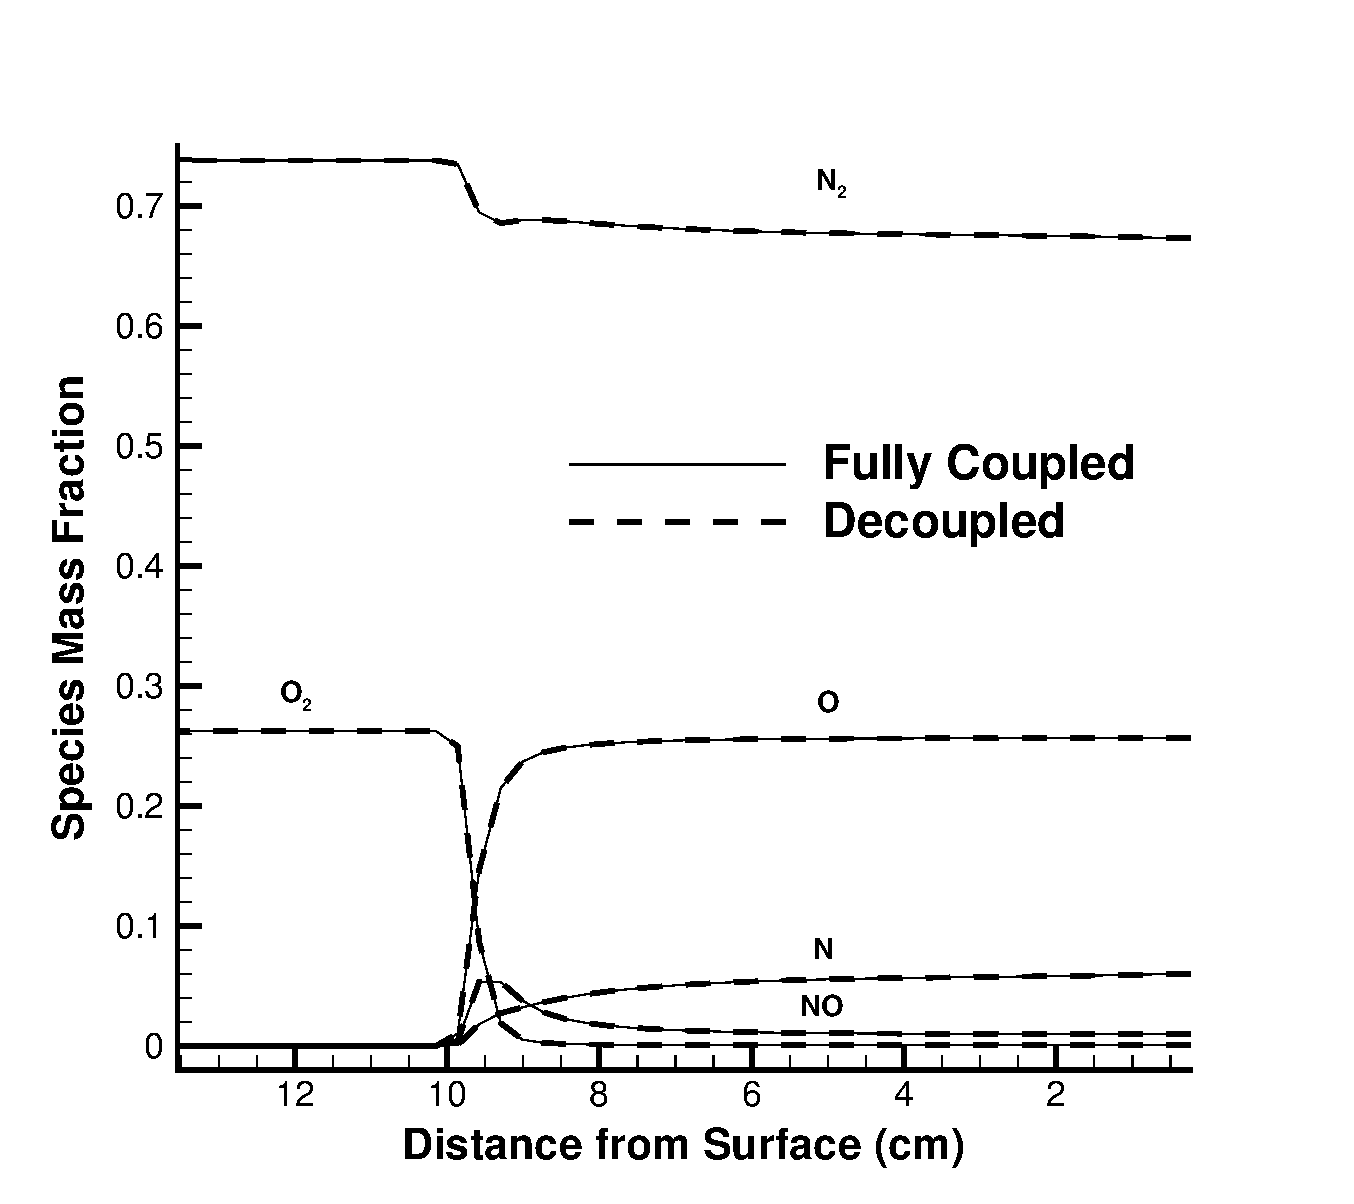
\includegraphics[width=\textwidth,trim={0 0 0 2cm}]{figures/stag_line_mf}
          \end{figure}
        \end{column}
      \end{columns}
      \vspace{3mm}
      \item Surface pressure, surface temperature, and mass fractions on
        stagnation line agree between decoupled and fully coupled
        implementations
    \end{itemize}
  \end{itemize}
\end{frame}
\begin{frame}
  \frametitle{Numerical Results: 2D Cylinder}
  \begin{columns}[t]
    \begin{column}{0.5\textwidth}
    \begin{figure}[h]
      \centering
      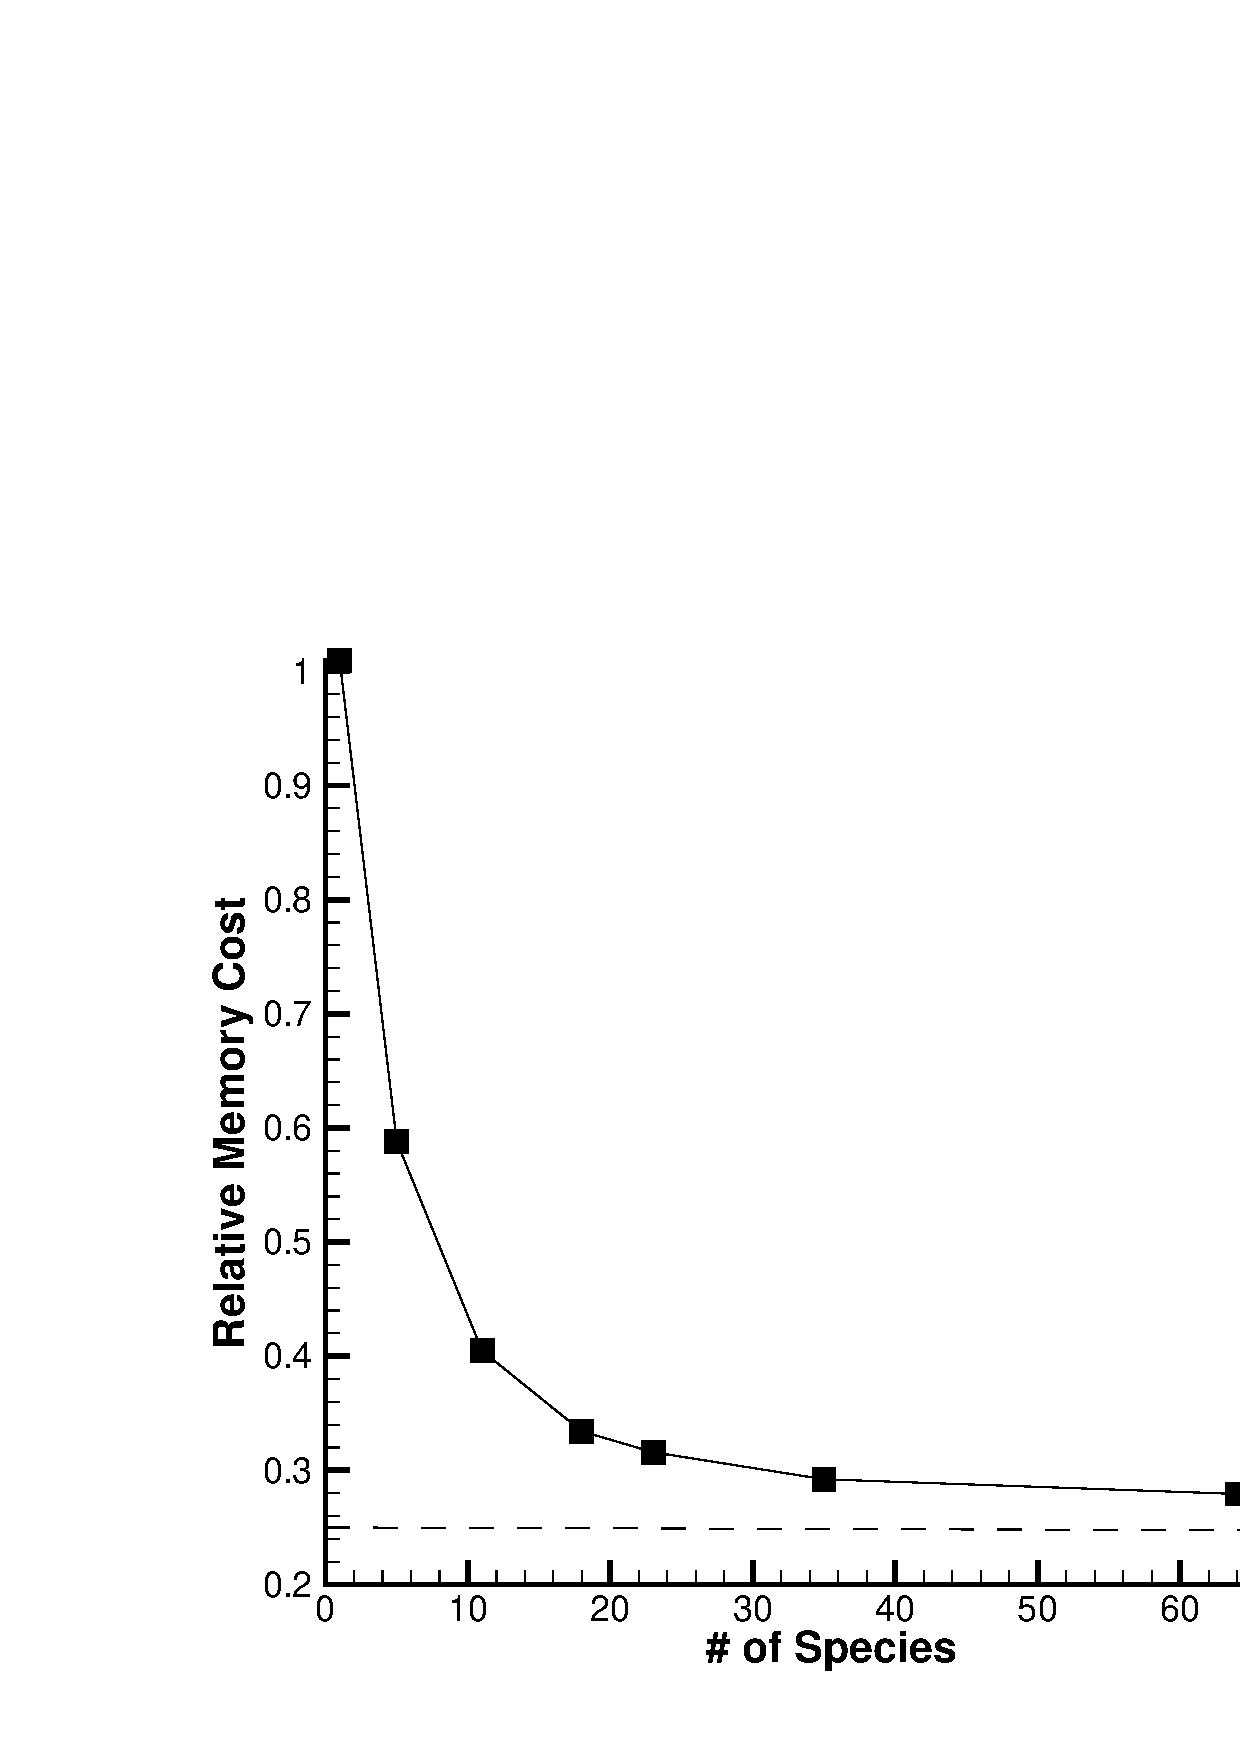
\includegraphics[width=0.8\textwidth,trim={0 0 1cm 2.5cm}]{figures/mem_req}
    \end{figure}
    \end{column}
    \begin{column}{0.5\textwidth}
      \begin{figure}[h]
        \centering
        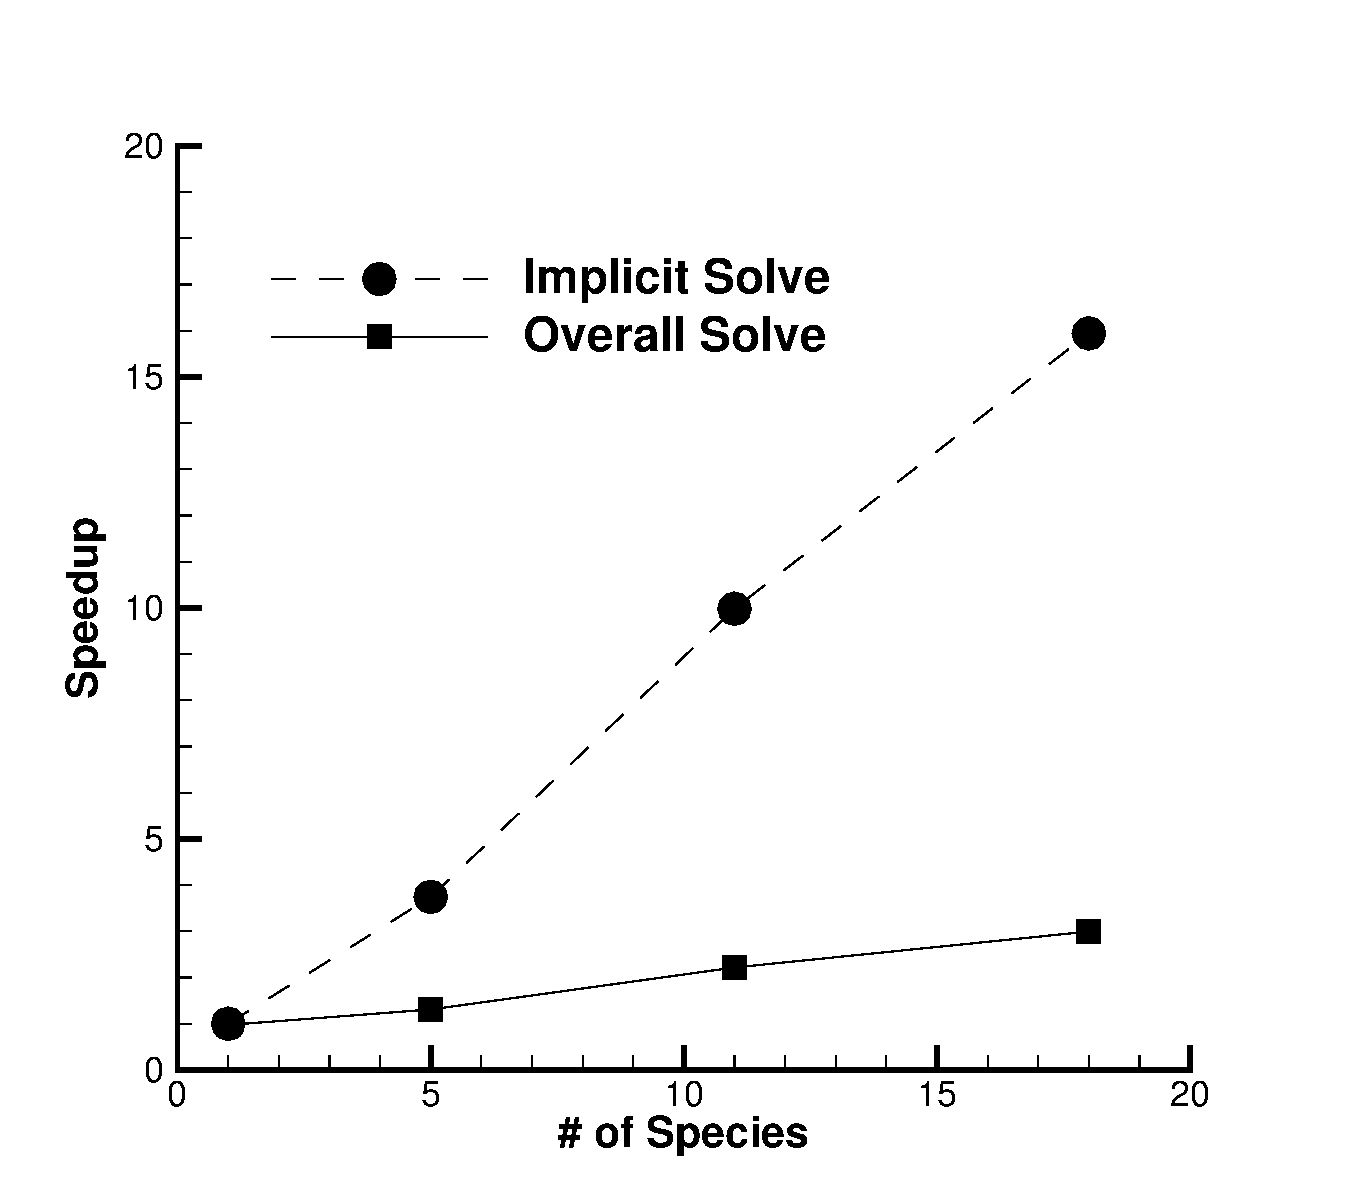
\includegraphics[width=0.8\textwidth,trim={1cm 0 0 2.5cm}]{figures/speedup} 
      \end{figure}
    \end{column}
  \end{columns}
  \begin{itemize}
    \item On structured grids $N_{nbrs} \approx 6 N_{nodes}$
    \begin{itemize}
      \item Half precision off-diagonal $N_{nbrs} = \frac{6N_{nodes}}{2}$
        \[ 
          Memory\ Cost \approx 
           \frac{N_{nodes}}{N_{nodes} + N_{nbrs}} =
           \frac{N_{nodes}}{N_{nodes} + 6N_{nodes}/2} = \frac{1}{4}
        \]
      \item Linear speedup in solver: $\frac{O(ns^2)}{O(ns)} = O(ns)$
    \end{itemize}
  \end{itemize}
\end{frame}

\subsection{Numerical Results: Axisymmetric Spherically Capped Cone}

\begin{frame}
  \frametitle{Numerical Results: Axisymmetric Spherically Capped Cone}
  \begin{figure}[h]
  	\centering
   \adjincludegraphics[width=0.6\textwidth,trim={0 3.5cm 0 3cm},clip]{figures/cone_mesh}
  \end{figure}
  \begin{itemize}
    \item Verify that the decoupled scheme is robust at high velocities
    \begin{itemize}
      \item $V_{\infty} = 15000\ m/s$, $\rho_{\infty}=0.001\ kg/m^3$, 
        $T_\infty = 200\ K$.
      \item 11-species air model N, $\text{N}_2$, O,
        $\text{O}_2$, NO, N$^+$, $\text{N}_2^+$, O$^+$, 
        $\text{O}_2^+$, NO$^+$, and electrons, with 22 possible reactions.
      \item Inviscid flow, with 1-Temperature model
    \end{itemize}
  \end{itemize}
\end{frame}
\begin{frame}
  \frametitle{Numerical Results: Axisymmetric Spherically Capped Cone}
    \begin{columns}[t]
      \begin{column}{0.5\textwidth}
        \begin{figure}[h!]
          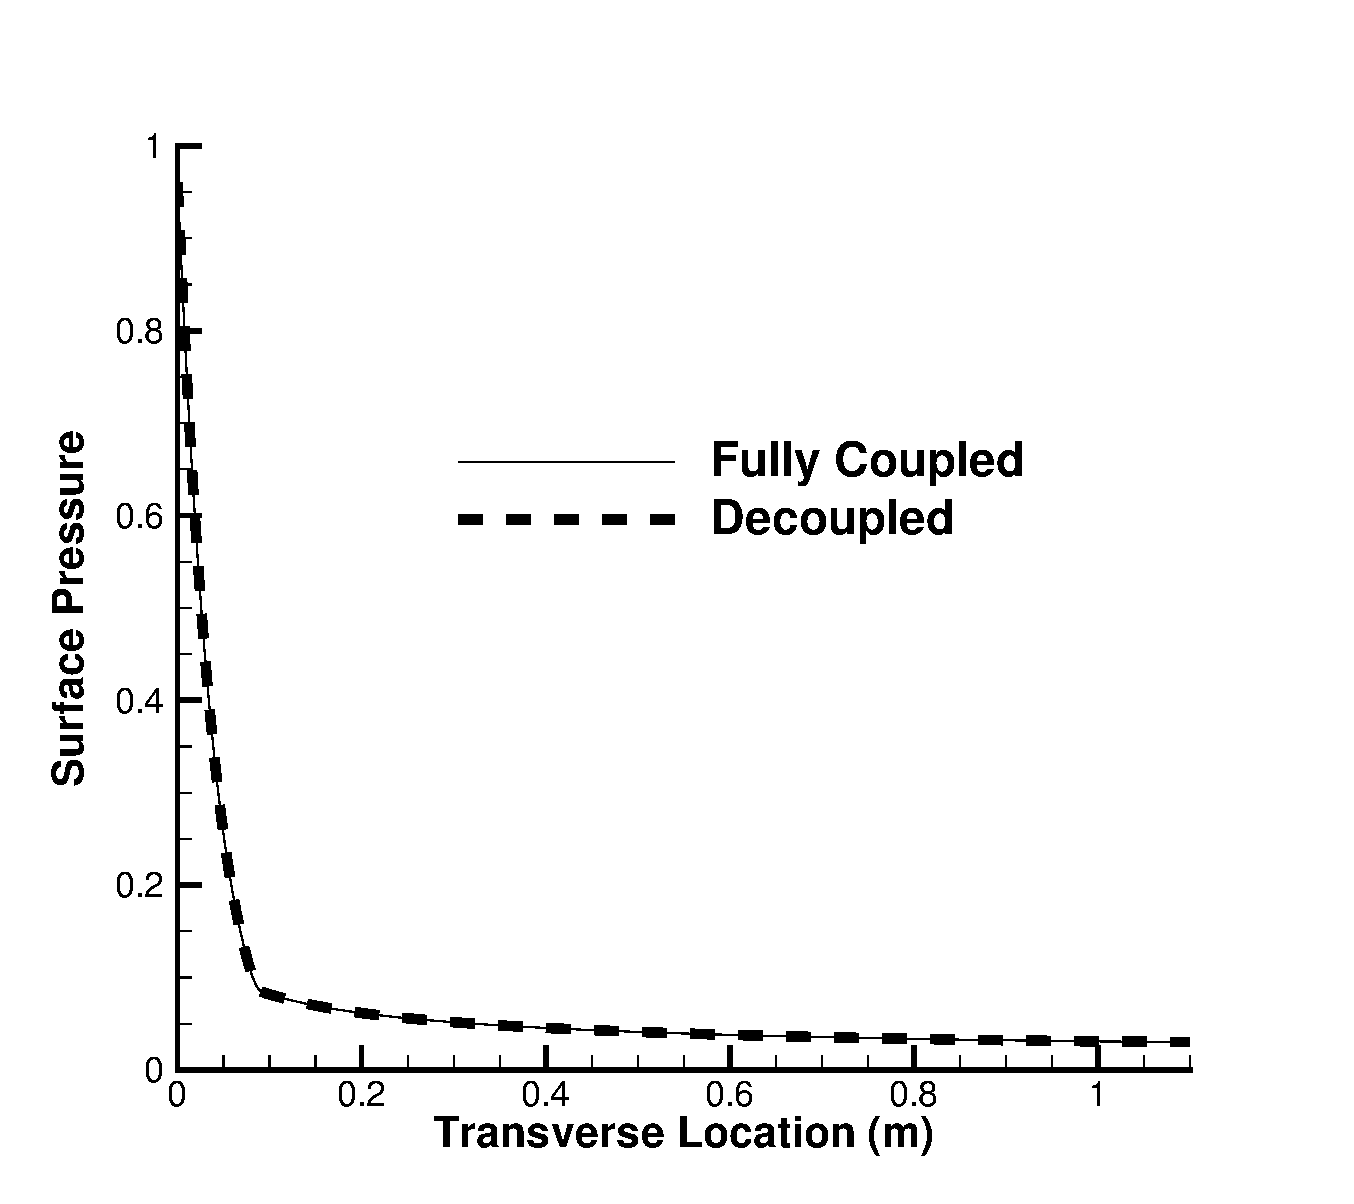
\includegraphics[width=\textwidth]{figures/surface_pressure_cone}
        \end{figure}
      \end{column}
      \begin{column}{0.5\textwidth}
        \begin{figure}[h!]
          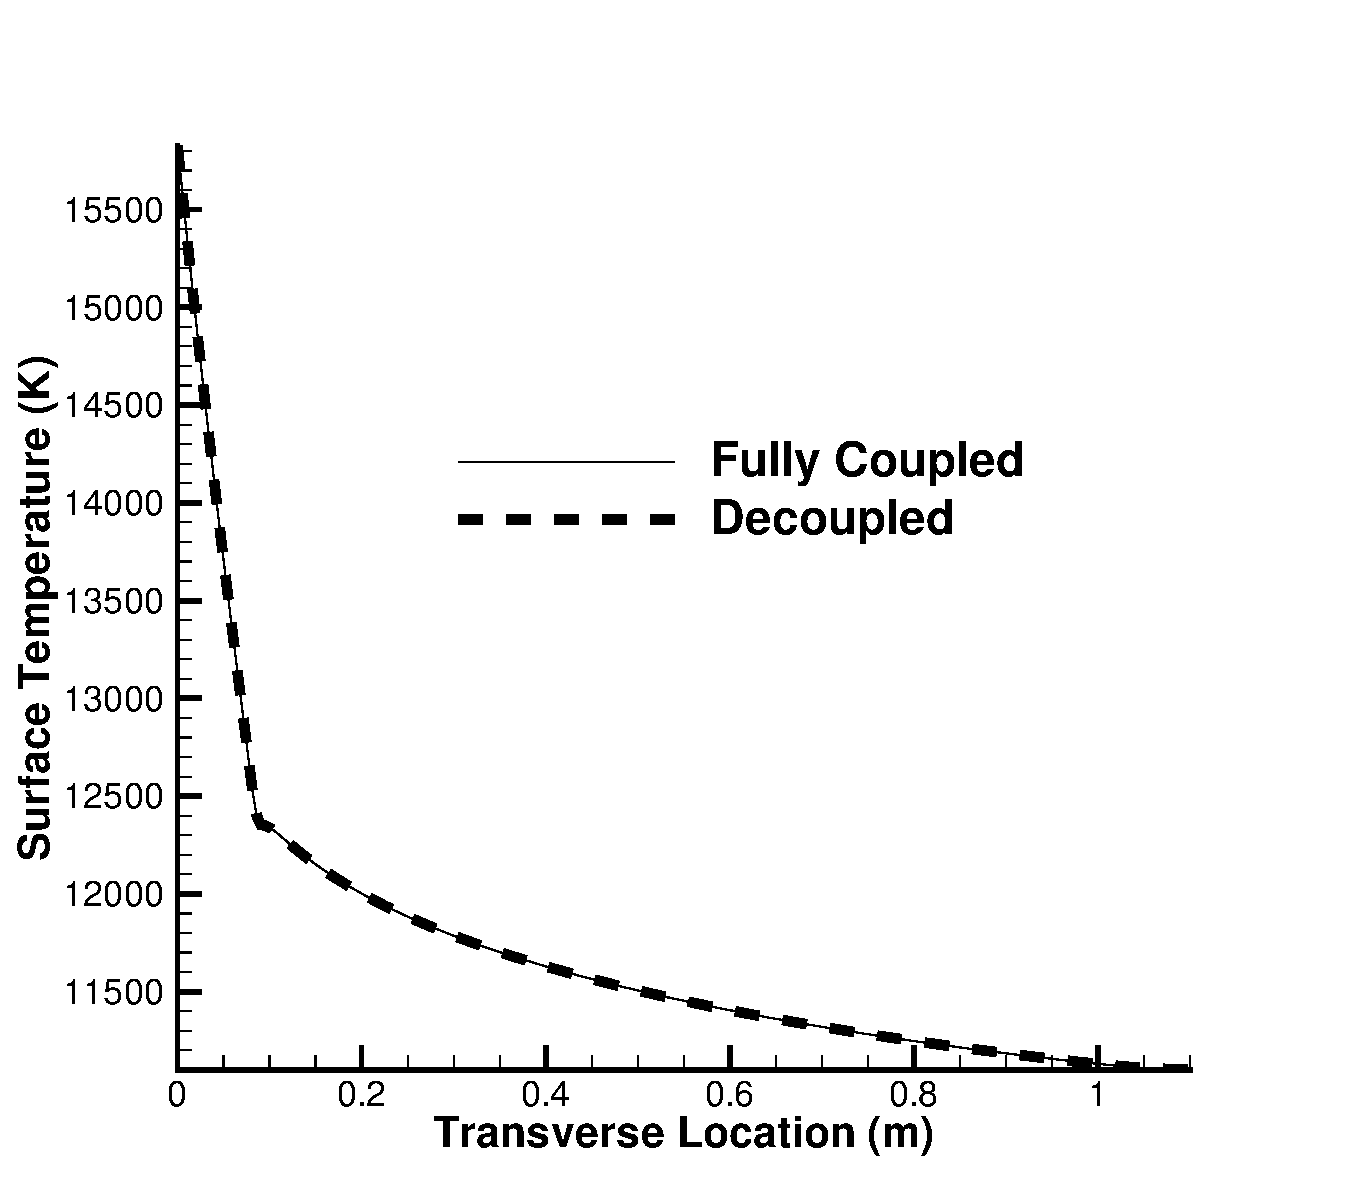
\includegraphics[width=\textwidth]{figures/surface_temperature_cone}
        \end{figure}
      \end{column}
    \end{columns}
    \begin{itemize}
      \item Surface pressure and surface temperature agree between decoupled and
        fully coupled implementations
    \end{itemize}
\end{frame}
\begin{frame}
  \frametitle{Numerical Results: Axisymmetric Spherically Capped Cone}
    \begin{columns}[t]
      \begin{column}{0.5\textwidth}
        \begin{figure}[h!]
    	  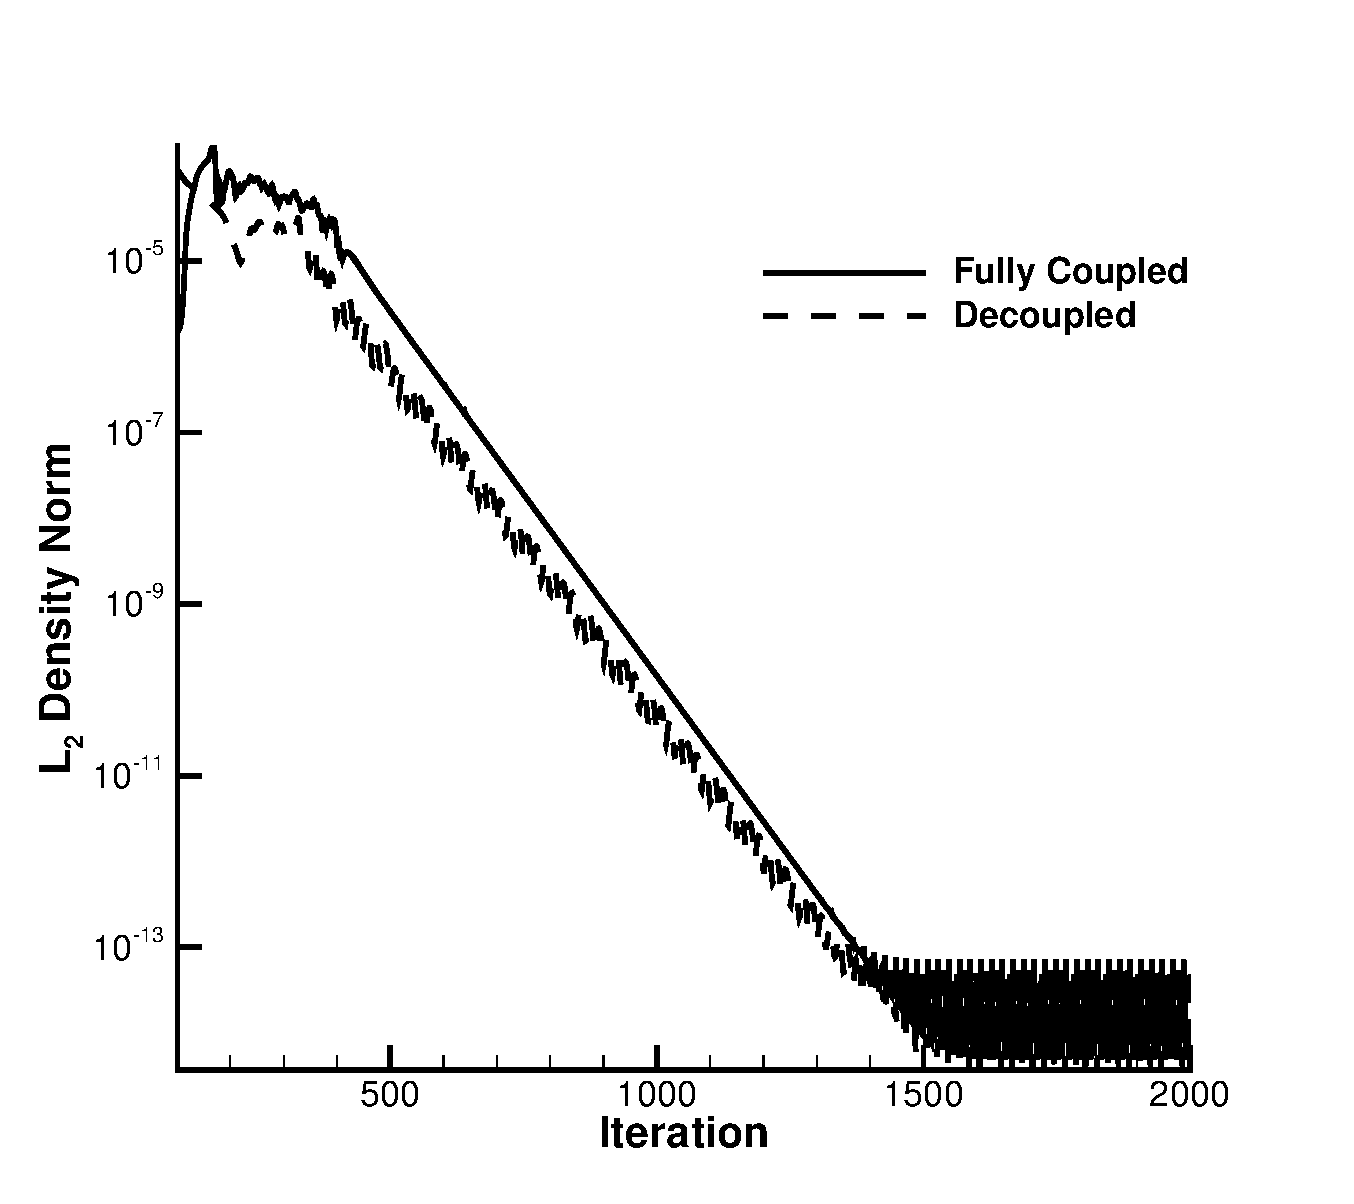
\includegraphics[width=\textwidth]{figures/cone_iteration}
        \end{figure}
      \end{column}
      \begin{column}{0.5\textwidth}
        \begin{figure}[h!]
	  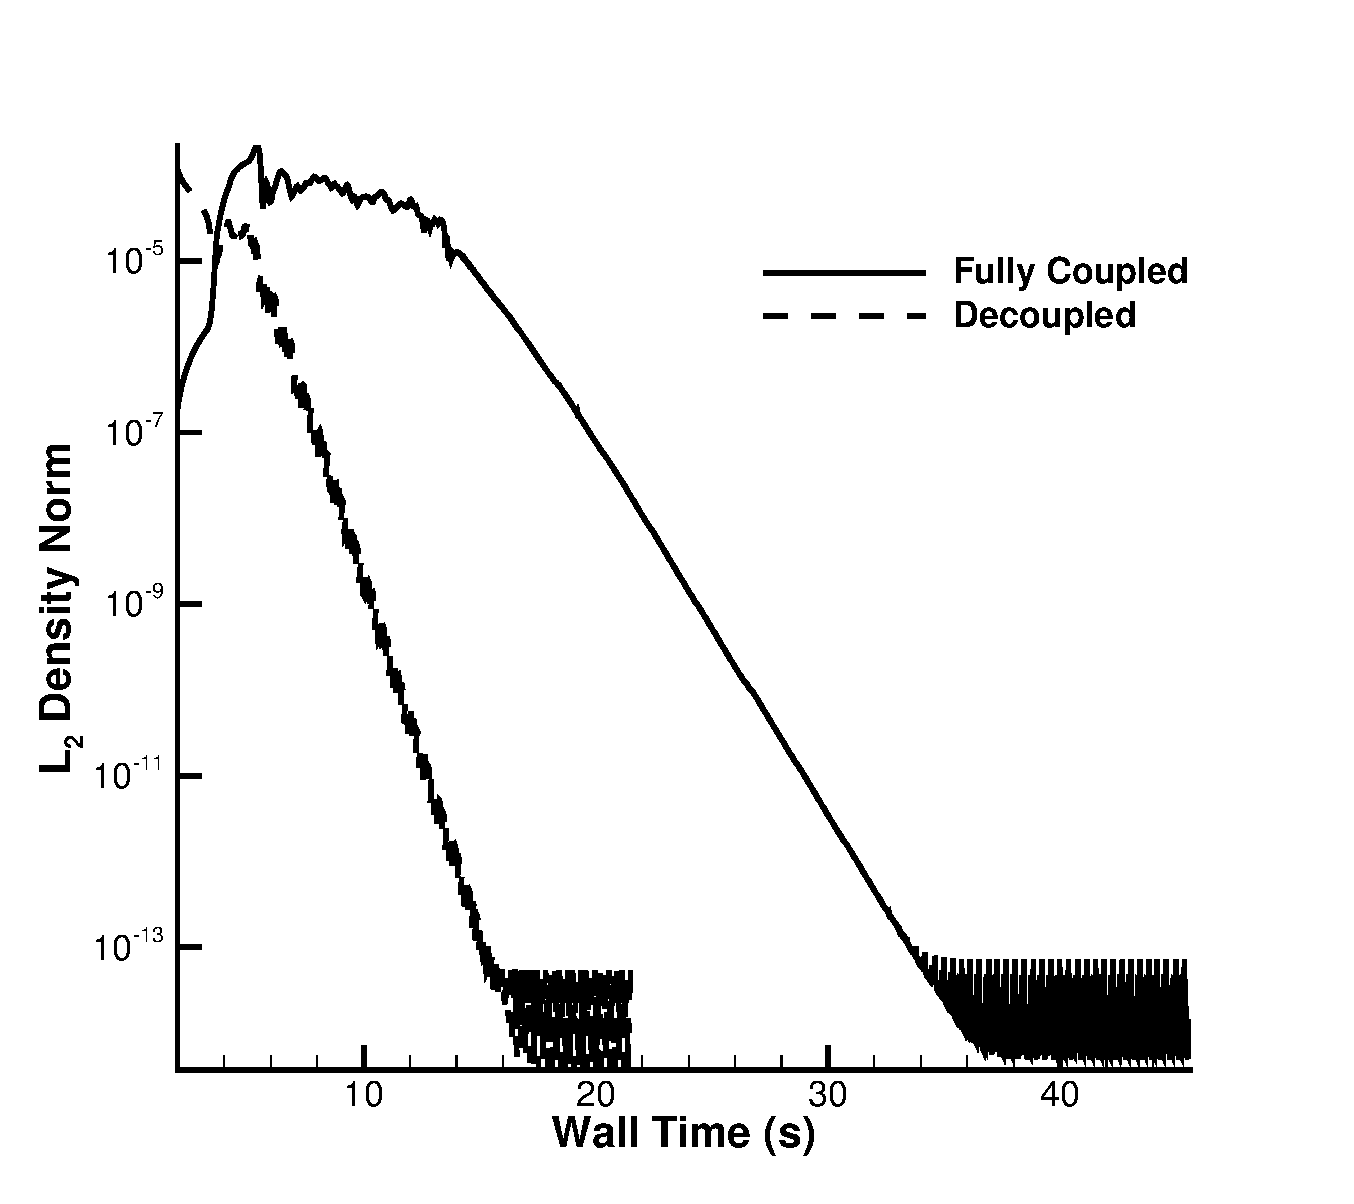
\includegraphics[width=\textwidth]{figures/cone_walltime}
        \end{figure}
      \end{column}
    \end{columns}
  \begin{itemize}
    \item Necessary to scale source term magnitude by $0.001 \leq w \leq 1$ 
      for the first 500 iterations, due to extreme reaction rates
    \item Both schemes converge in a similar number of iterations
    \item Decoupled scheme $\approx$ 2x faster
  \end{itemize}
\end{frame}


\section{Linearization Schemes Review}
\stepcounter{subsection}
\begin{frame}
  \frametitle{Linearization Schemes Review}
  \begin{itemize}
    \item Decoupled scheme based on work by Candler, et. al\footnotemark
    \item Main idea is to ``decouple'' the conserved variable vector, $\mU$,
      into mixture, $\mUp$, and species, $\Vhat$, variable vectors
      \begin{equation}
      	\mU=\begin{pmatrix}
         	\rho_1\\
      		\vdots \\
      		\rho_{N_s} \\
      		\rho u \\
      		\rho v \\
      		\rho w \\
      		\rho E \\
      	\end{pmatrix}
        \rightarrow
      	\mUp=\begin{pmatrix}
         	\rho   \\
      		\rho u \\
      		\rho v \\
      		\rho w \\
      		\rho E \\
      	\end{pmatrix}
        ,\ 
      	\Vhat=\begin{pmatrix}
         	c_1\\
      		\vdots \\
      		c_{N_s} \\
      	\end{pmatrix}
       \end{equation}
       \begin{equation*}
         c_s = \frac{\rho_s}{\rho}, \quad N_s = \text{Number of species}
       \end{equation*}
  \end{itemize}
  \footnotetext[1]{Graham V. Candler, Pramod K. Subbareddy, and Ioannis Nompelis.
  "Decoupled Implicit Method for Aerothermodynamics and Reacting Flows", AIAA
  Journal, Vol. 51, No. 5 (2013), pp. 1245-1254.}
\end{frame}
\stepcounter{subsection}
\begin{frame}
  \frametitle{Linearization Schemes Review}
  \tiny
  \begin{equation*}
    \label{dc_sys} 
    \begin{pmatrix} 
      \Box & & & & \\ & \ddots & & & \\ & & \Box \\ & & & \ddots & \\ & & & & \Box
    \end{pmatrix}
    \begin{pmatrix}
      \delta \mathbf{\hat{V}}_1 \\ \vdots \\ \delta \mathbf{\hat{V}}_i \\ 
      \vdots \\ \delta \mathbf{\hat{V}}_{nodes}
    \end{pmatrix}
    =
    \begin{pmatrix}
      \hat{b}_1 \\ \vdots \\ \hat{b}_i \\ \vdots \\ \hat{b}_{nodes} 
    \end{pmatrix}
    -
    \begin{pmatrix}
      (\sum_{j=1}^{N_{nb}}{[\diagdown] \delta\mathbf{\hat{V}}_{j}})_1 \\ \vdots \\
      (\sum_{j=1}^{N_{nb}}{[\diagdown] \delta\mathbf{\hat{V}}_{j}})_i \\ \vdots \\
      (\sum_{j=1}^{N_{nb}}{[\diagdown] \delta\mathbf{\hat{V}}_{j}})_{nodes}
    \end{pmatrix} 
  \end{equation*} 
  \normalsize
  \begin{itemize}
    \item Cost and memory saving for decoupled scheme stem from decoupled mass
      fraction block Jacobians, $\pd{R}{\Vhat}$, being diagonal for convective
      flux.
      \begin{itemize}
        \item Linear solve reduced from $O(N_{s}^2) \rightarrow O(N_{s})$
        \item Relative memory savings between decoupled and fully-coupled
          linearization schemes (for structured-type grid)\footnotemark
          \begin{equation}
            \lim_{N_s \rightarrow \infty} \frac{\text{decoupled memory req.}}
            {\text{fully coupled memory req.}} = \frac{1}{7}
            \label{mem-savings}
          \end{equation}
      \end{itemize}
  \end{itemize}
  \footnotetext[2]{Relative memory savings theoretically greater for tetrahedral
  grids}
\end{frame}
\section{Demonstration Problem: Annular Nozzle}
\stepcounter{subsection}
\begin{frame}
  \frametitle{Annular Nozzle - Geometry}
  \begin{columns}
    \begin{column}{0.4\textwidth}
     \begin{figure}
       \centering
        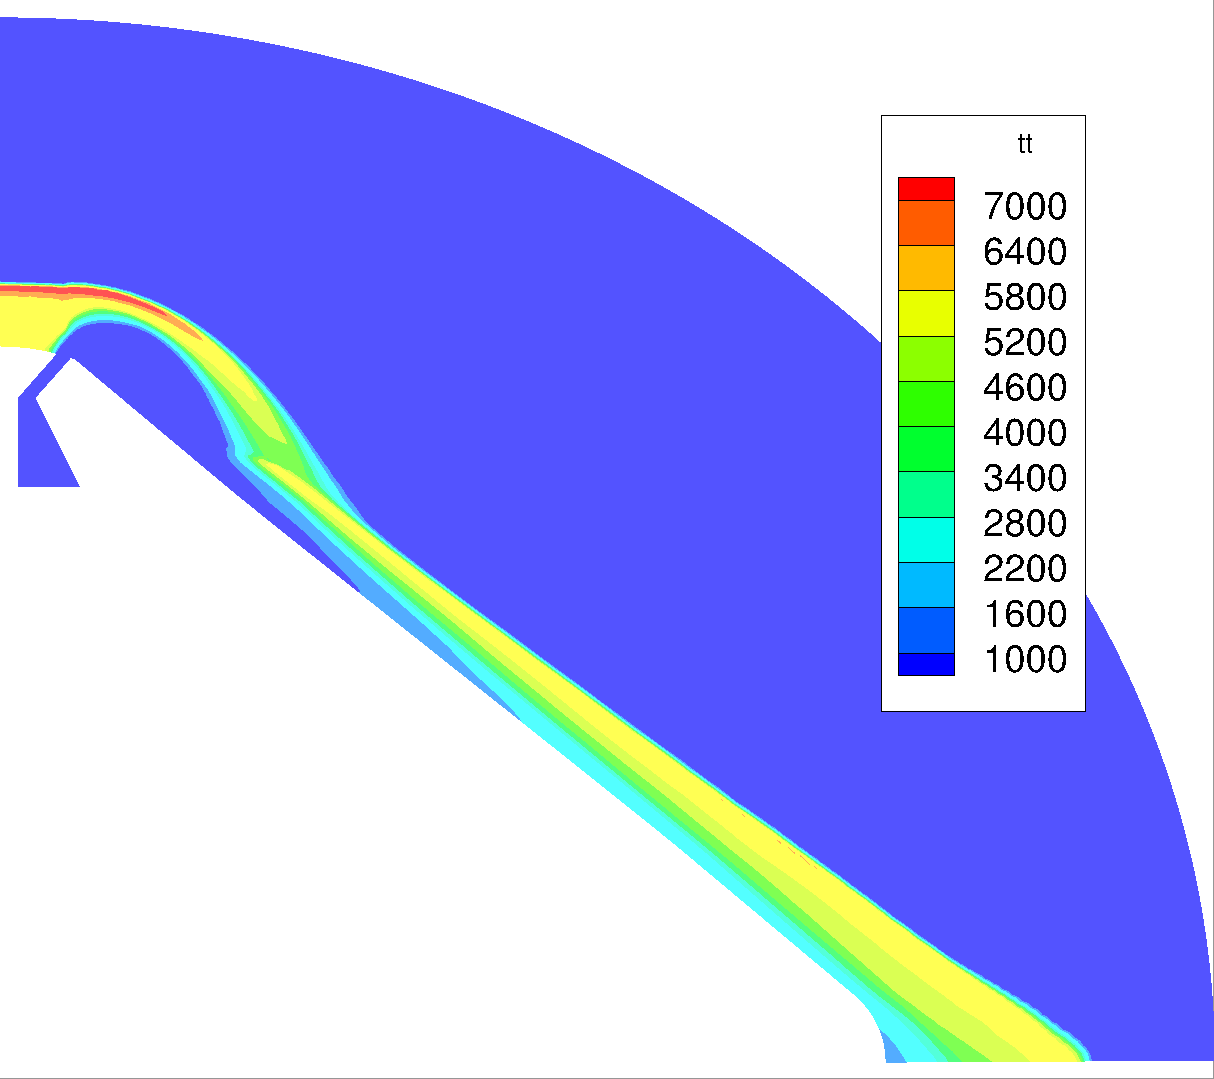
\includegraphics[width=\textwidth]{figures/flow-viz.png}
       \caption{Annular Jet Temperature Contours}
       \label{fig:annular-jet-flow}
     \end{figure}
    \end{column}
    \begin{column}{0.6\textwidth}
      \begin{table}
        \tiny
        \centering
        \begin{tabular}{c|c|c}
          Flow Condition & Description & Value \\
          \hline
          $V_{\infty}$    & freestream velocity, $m/s$        & 5686.24 \\
          $\rho_{\infty}$ & freestream density, $kg/m^3$      & 0.001 \\
          $T_{\infty}$    & freestream temperature, $K$       & 200.0 \\
          $M_{\infty}$    & freestream Mach number (derived)  & 20.0
        \end{tabular}
        \caption{Flow Conditions}
        \label{tab:flow-conditions}
      \end{table}
      \begin{table}
       \tiny
        \centering
        \begin{tabular}{c|c|c}
          Parameter & Description & Value \\
          \hline
          $r_{throat}$       &   nozzle throat radius, $m$           & 0.02 \\
          $r_{plenum}$       &   nozzle radius at plenum face, $m$   & 0.05 \\
          $r_{exit,inner}$   &   inside nozzle radius at exit, $m$   & 0.05 \\
          $r_{exit,outer}$   &   outside nozzle radius at exit, $m$  & 0.07 \\
          $l_{conv}$         &   distance from plenum to throat, $m$ & 0.05 \\
          $\theta_c$         &   cone half angle, deg                & 50.0
        \end{tabular}
        \caption{Annular Nozzle Geometry Inputs}
        \label{tab:annular-geom}
      \end{table}
    \end{column}
  \end{columns}
  \begin{itemize}
    \item Note: $50^o$ cone angle chosen to prevent sonic corner body
  \end{itemize}
\end{frame}
\begin{frame}
  \frametitle{Annular Nozzle - Flow Solver Cost Savings}
  \begin{itemize}
    \item Best case scenario: decoupled scheme 1st-order w/frozen flow
      \begin{columns}
        \begin{column}{0.4\textwidth}
          \centering
          \begin{figure}[h]
            \centering
            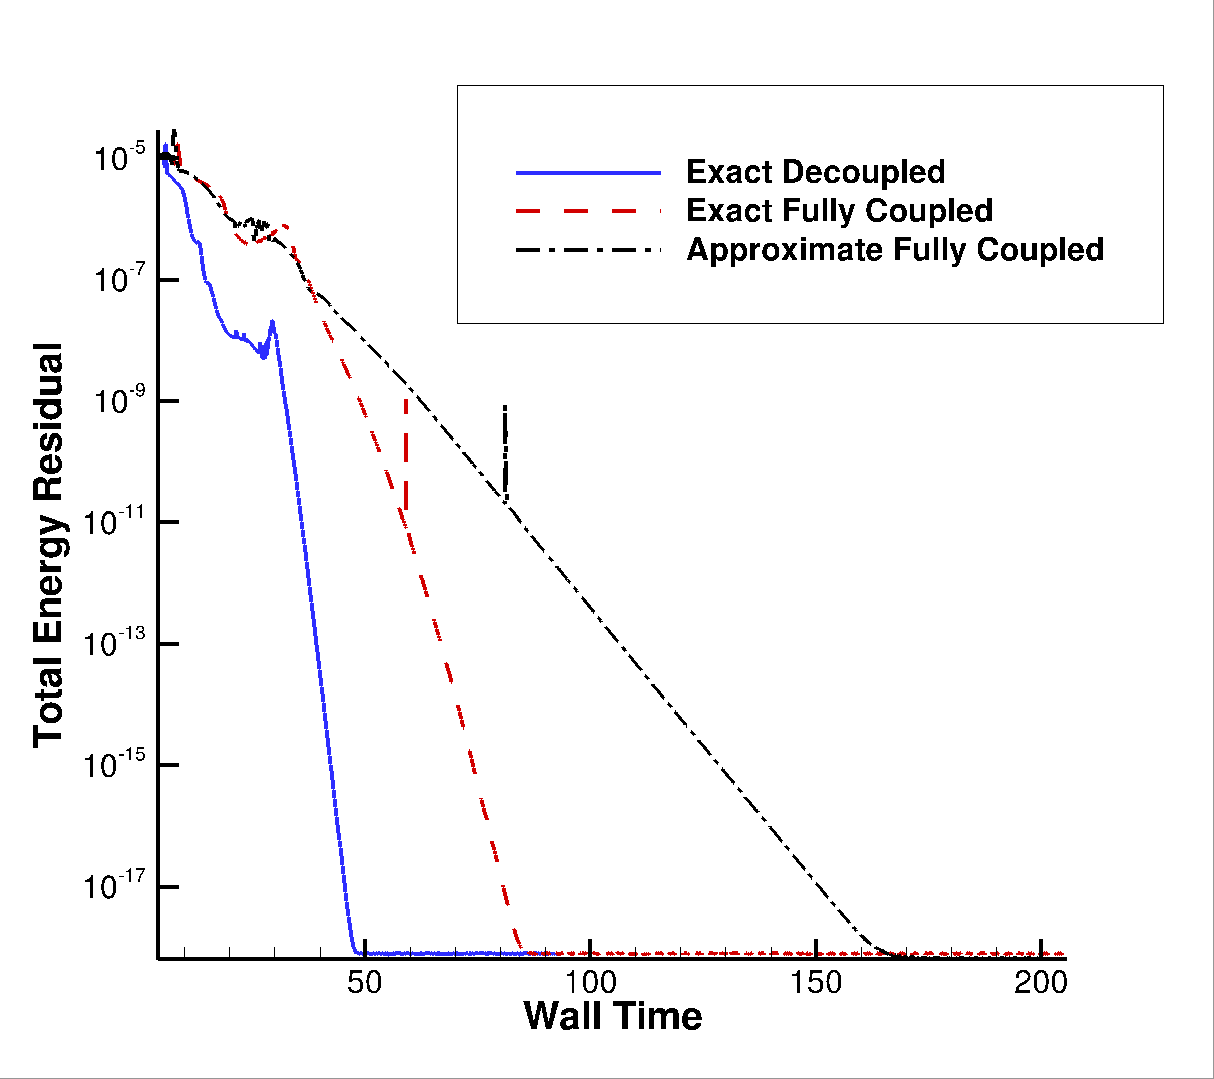
\includegraphics[width=\textwidth]{figures/1st-order.png}
            \caption{1st-Order Frozen Flow Convergence History}
            \label{fig:1st-order}
          \end{figure}
        \end{column}
        \begin{column}{0.6\textwidth}
          \centering
          \begin{table}
            \tiny
            \centering
            \begin{tabular}{c|c|c}
              Scheme & Time to Convergence (s) & Speedup \\
              \hline
              Approx. FC & 150.7 & 1.00 (baseline) \\
              Exact FC   & 80.71 & 1.87 \\
              Exact DC   & 45.60 & 3.30 \\
            \end{tabular}
            \caption{Speedup relative to the approximate, fully-coupled Jacobians}
            \label{tab:1st-order}
          \end{table}
          \vspace{-0.5cm}
          \begin{itemize}
            \item CFL ramped from $0.1 \rightarrow 30.0$ for all schemes
            \item Exact linearizations significantly improve the rate of
              convergence after non-linear transients of startup
          \end{itemize}
        \end{column}
      \end{columns}
  \end{itemize}
\end{frame}
\begin{frame}
  \frametitle{Annular Nozzle - Inverse Design Optimization}
  \vspace{-0.5cm}
  \begin{columns}
    \begin{column}{0.5\textwidth}
      \centering
      \begin{figure}[h]
        \centering
        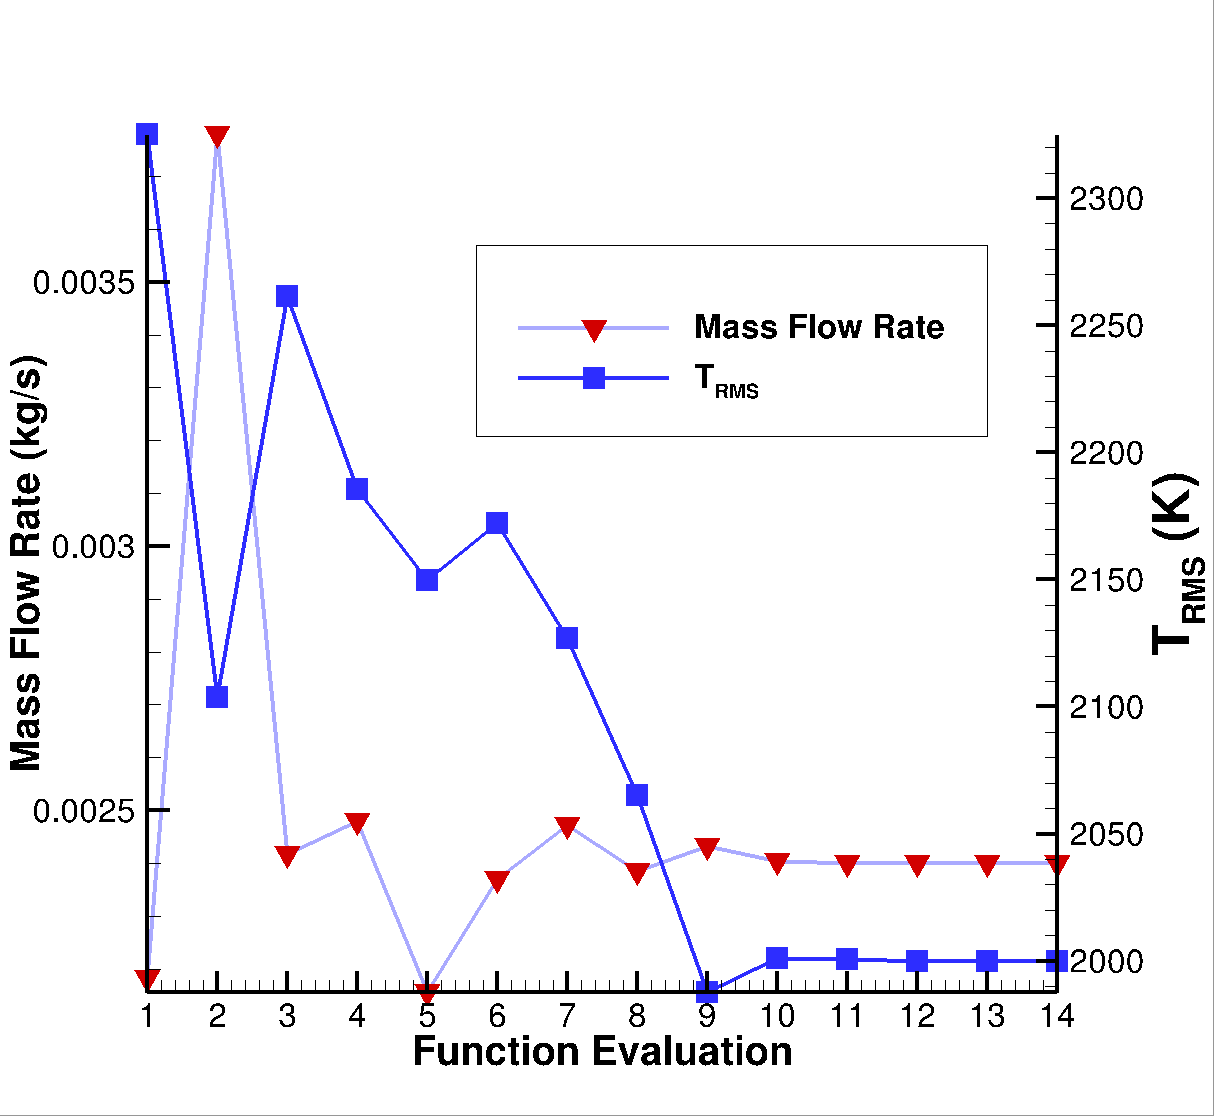
\includegraphics[width=\textwidth]{figures/1st-H2/fm_hist.png}
        \caption{Temperature and mass flow rate design history}
        \label{fig:fm-hist}
      \end{figure}
    \end{column}
    \begin{column}{0.5\textwidth}
      \centering
      \begin{figure}[h]
        \centering
        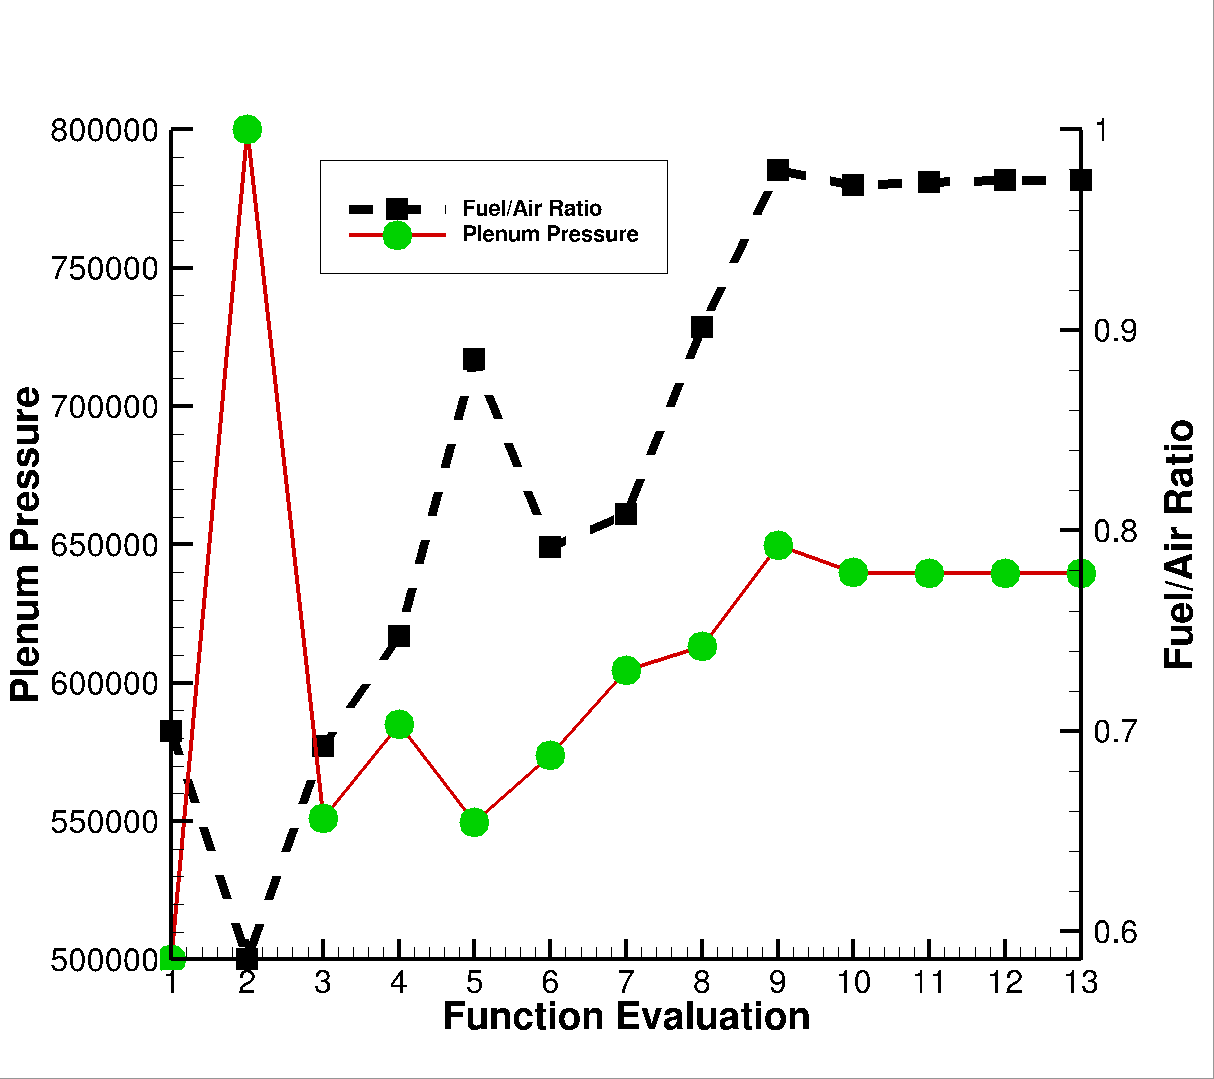
\includegraphics[width=\textwidth]{figures/1st-H2/dv_hist.png}
        \caption{Design variable history}
        \label{fig:dv-hist}
      \end{figure}
    \end{column}
  \end{columns}
  \begin{itemize}
    \item Plenum pressure and $H_2$/$N_2$ ratio chosen as design variables
    \item Design to within $10^{-4}$ of target by 11 Flow/Adjoint solves
  \end{itemize}
\end{frame}
\section{Concluding Remarks}
\stepcounter{subsection}
\begin{frame}
  \frametitle{Concluding Remarks}
  \begin{itemize}
    \item 1st-order inverse and direct design optimization very robust for
      annular jet
    \item Decoupled linearizations very robust, and typically can be run with
      same options as fully-coupled schemes.  
      \begin{itemize}
        \item Source term scaling is still needed for intense chemical reactions
          (i.e.  combustion, full $N_2$ dissociation, etc.)
        \item 2nd-order has more complicated history, but 2x speed is generally
          recovered by the decoupled scheme over approximate and exact fully coupled
          schemes
      \end{itemize}
    \item Fully coupled adjoint robust, and costs $\sim \frac{1}{2}$ flow
      solution cost
      \begin{itemize}
        \item Decoupled adjoint yields both super-convergence and divergence.  Still
          under investigation.
      \end{itemize}
  \end{itemize}
\end{frame}
\section{}
\begin{frame}
  \frametitle{Backup - Annular Nozzle Direct Design}
  \begin{columns}
    \begin{column}{0.4\textwidth}
      \begin{figure}[h]
        \centering
        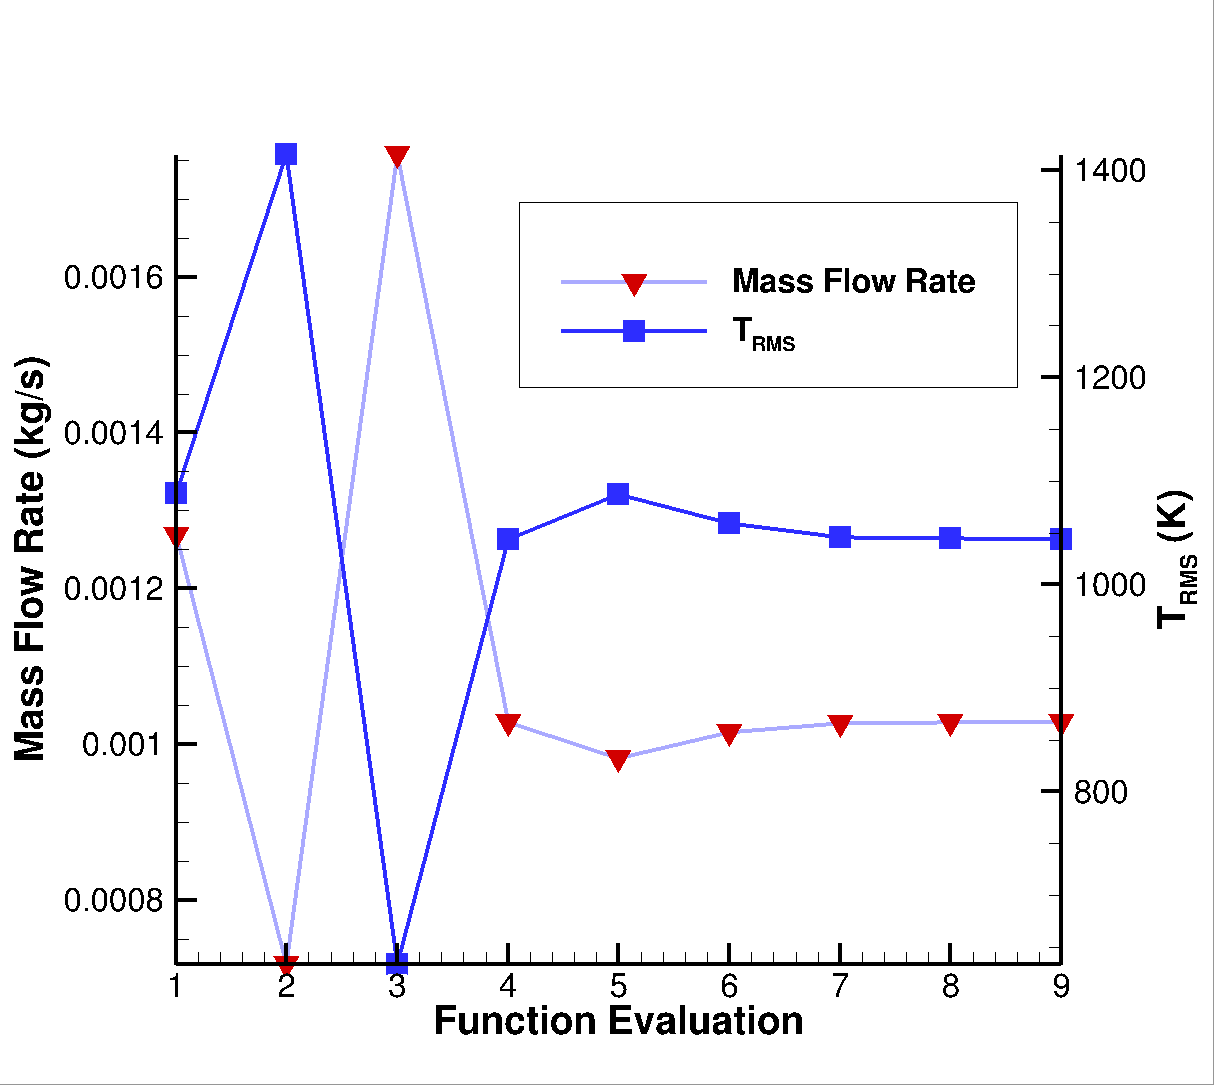
\includegraphics[width=\textwidth]{figures/direct_design/mass-tt.png}
        \caption{Temperature and mass flow rate design history}
        \label{fig:dd-temp-mass}
      \end{figure}
    \end{column}
    \begin{column}{0.6\textwidth}
      \begin{itemize}
        \item Cost function definition
          \begin{gather*}
            f = w_1 \left( T_{RMS} \right)^2 + w_2 \left( \dot{m} \right)^2 \\
            \frac{w_1}{w_2} = 
            \frac{\left (T_{RMS} \right)^2}{\left(\dot{m} \right)^2}
            \label{cost-func}
          \end{gather*}
        \item Net design improved by $9.3\%$
          \begin{table}
            \tiny
            \centering
            \begin{tabular}{c|c|c|c}
              Component & Initial & Final & Improvement\\
              \hline
              $\dot{m}$, $kg/s$ & 1.268e-3 & 1.327e-3 & -4.6\% \\
              $T_{RMS}$, $K$ & 2473        & 2132     & 13.79\%
            \end{tabular}
            \caption{Design Improvement}
            \label{tab:design-improvement}
          \end{table}
      \end{itemize}
    \end{column}
  \end{columns}
\end{frame}
\begin{frame}
  \frametitle{Backup - Adjoint Convergence}
  \begin{columns}
    \begin{column}{0.5\textwidth}
      \begin{figure}[h]
        \centering
        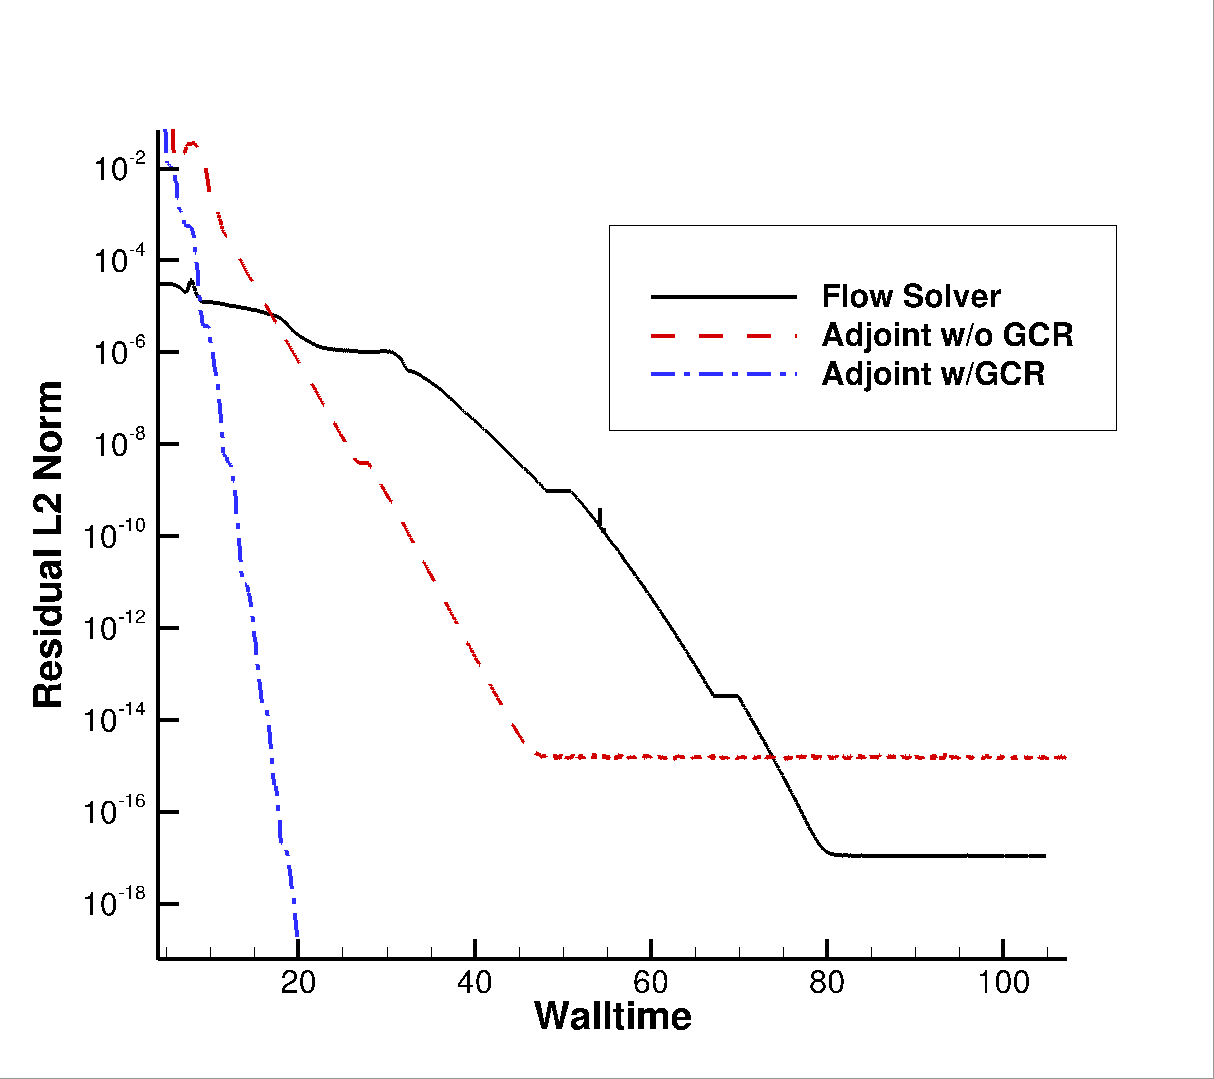
\includegraphics[width=\textwidth]{figures/adj-comp.png}
        \caption{1st-order Adjoint Convergence}
        \label{fig:adj-comp}
      \end{figure}
    \end{column}
    \begin{column}{0.5\textwidth}
      \begin{itemize}
        \item First order adjoint convergence for exact, fully-coupled
          linearizations converges in $\sim \frac{1}{2}$ the time required by
          the flow solver
        \item If krylov scheme (GCR) is used, the time required is 
          $\sim \frac{1}{4}$ the time required by the flow solver
      \end{itemize}
    \end{column}
  \end{columns}
\end{frame}
\end{document}
